\chapter{Ensamblaje e instrumentacion}

En este capitulo se presentaran todos los detalles del ensamblado del reflector parabolico, la instalacion del rotor y la integracion de estos con el soporte de la montura en el pedestal construido para el telescopio. Tambien se detallaran todos los instrumentos evaluados y seleccionados para la construccion del receptor de radiofrecuencia, el rack de control y la infraestructura de caracterizacion.\\

Junto con esto, se mosntraran todas las piezas diseñadas e impresas en 3D para el soporte del alimentador y todos los soportes especificos que se necesitaron para la instalacion de los distintos componentes del telescopio.\\

Para finalizar con la descripcion del software creado para la operacion, mantenimiento y caracterizacion del telescopio.\\

\section{Ensamblado Mecánico}

Tanto el reflector parabolico como la montura alt azimutal y su correspondiente controlador, son elementos adquiridos de la compañia \textit{RFHamdesign}, una empresa holandesa que se especializa en la construccion de telescopios de radio aficionados. El reflector de 3 metros venia completamente desarmado y con piezas que requerian ser modificadas y ensambladas para su correcto funcionamiento.\\

Para todo el ensamblado se utilizaron herramientas de y electricas, como taladors, tijeras de ojalata, remachadoras, etc.\\

\begin{figure}
    \centering
    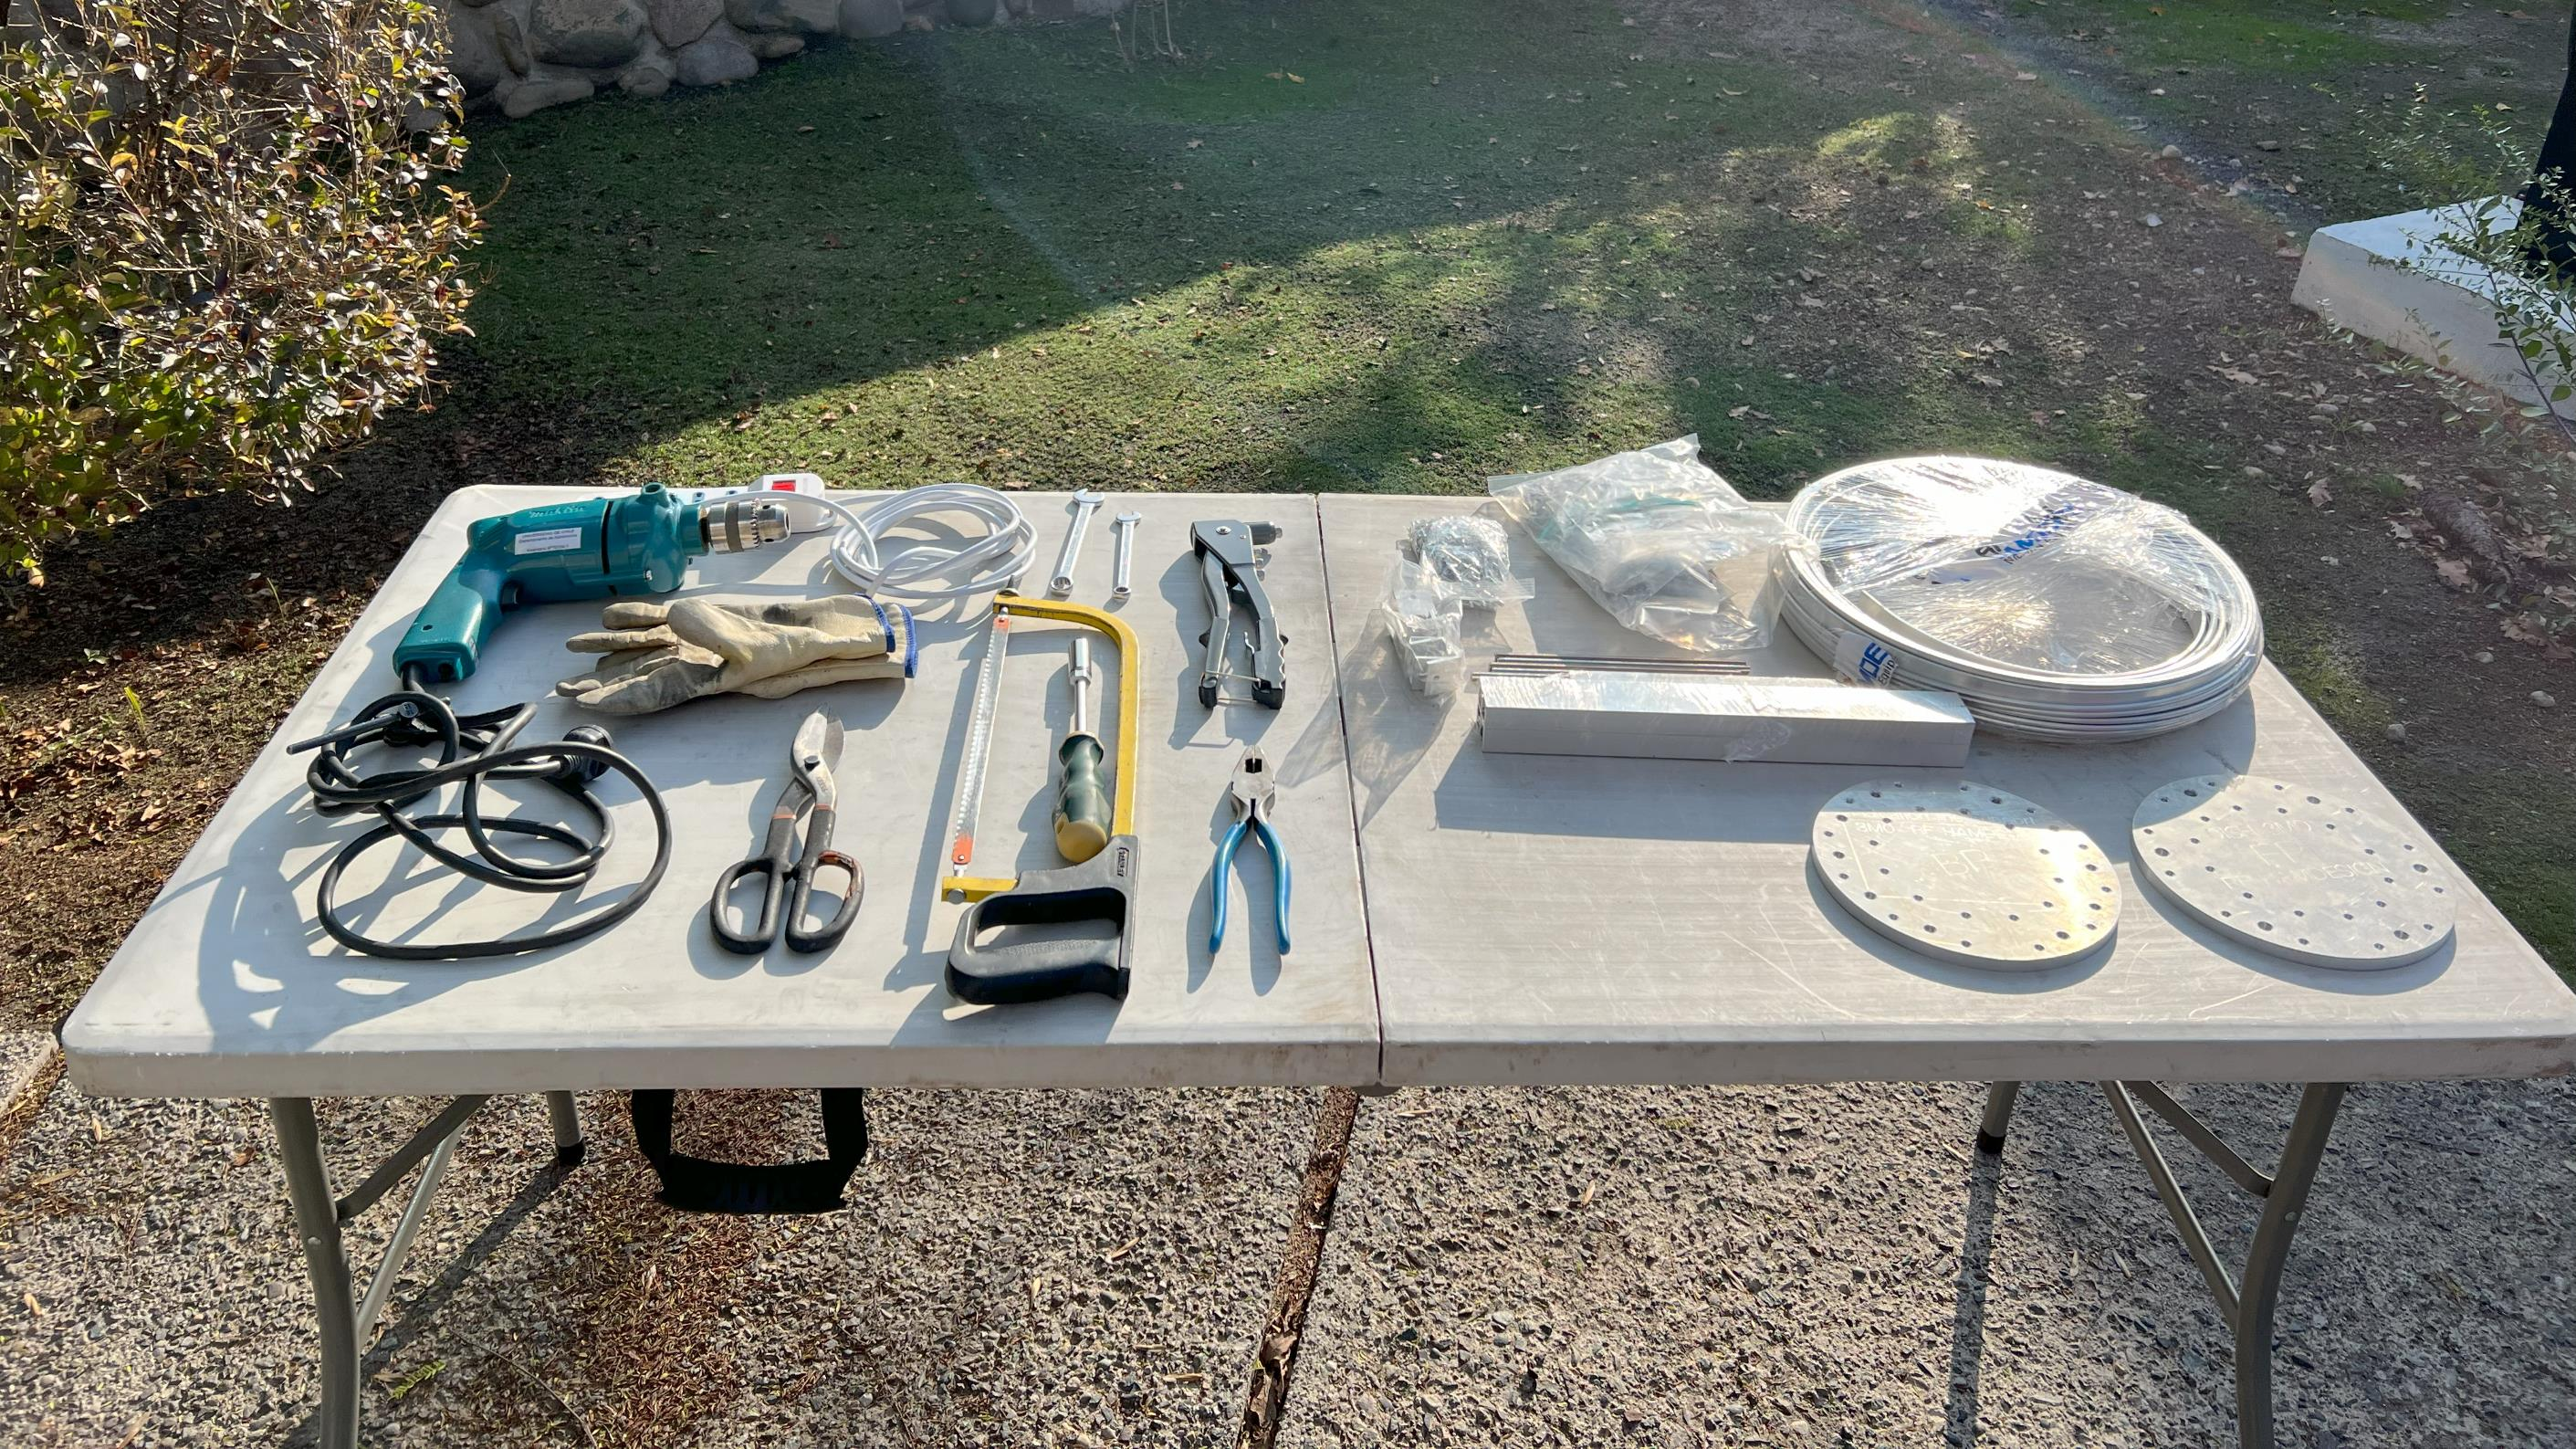
\includegraphics[width=0.8\textwidth]{img/herramientas}
    \caption{Herramientas utilizadas para el ensamblado de la superficie del reflector parabólico.}
    \label{fig:ensamblado1}
\end{figure}

En la figura \ref{fig:ensamblado1} se pueden ver las herramientas utilizadas para el ensamblado de la superficie del reflector parabólico ademas de las piezas que requerian de modificacion adicional para la instalacion correcta.\\

\subsection{Reflector Parabólico}

Las piezas del reflector se dividen en los 12 arcos, o costillas, de aluminio que conforman la estructura que da forma a la superficie parabolica, con un centro de aluminion donde estas 12 piezas se unen y apernan.\\

\begin{figure}
    \centering
    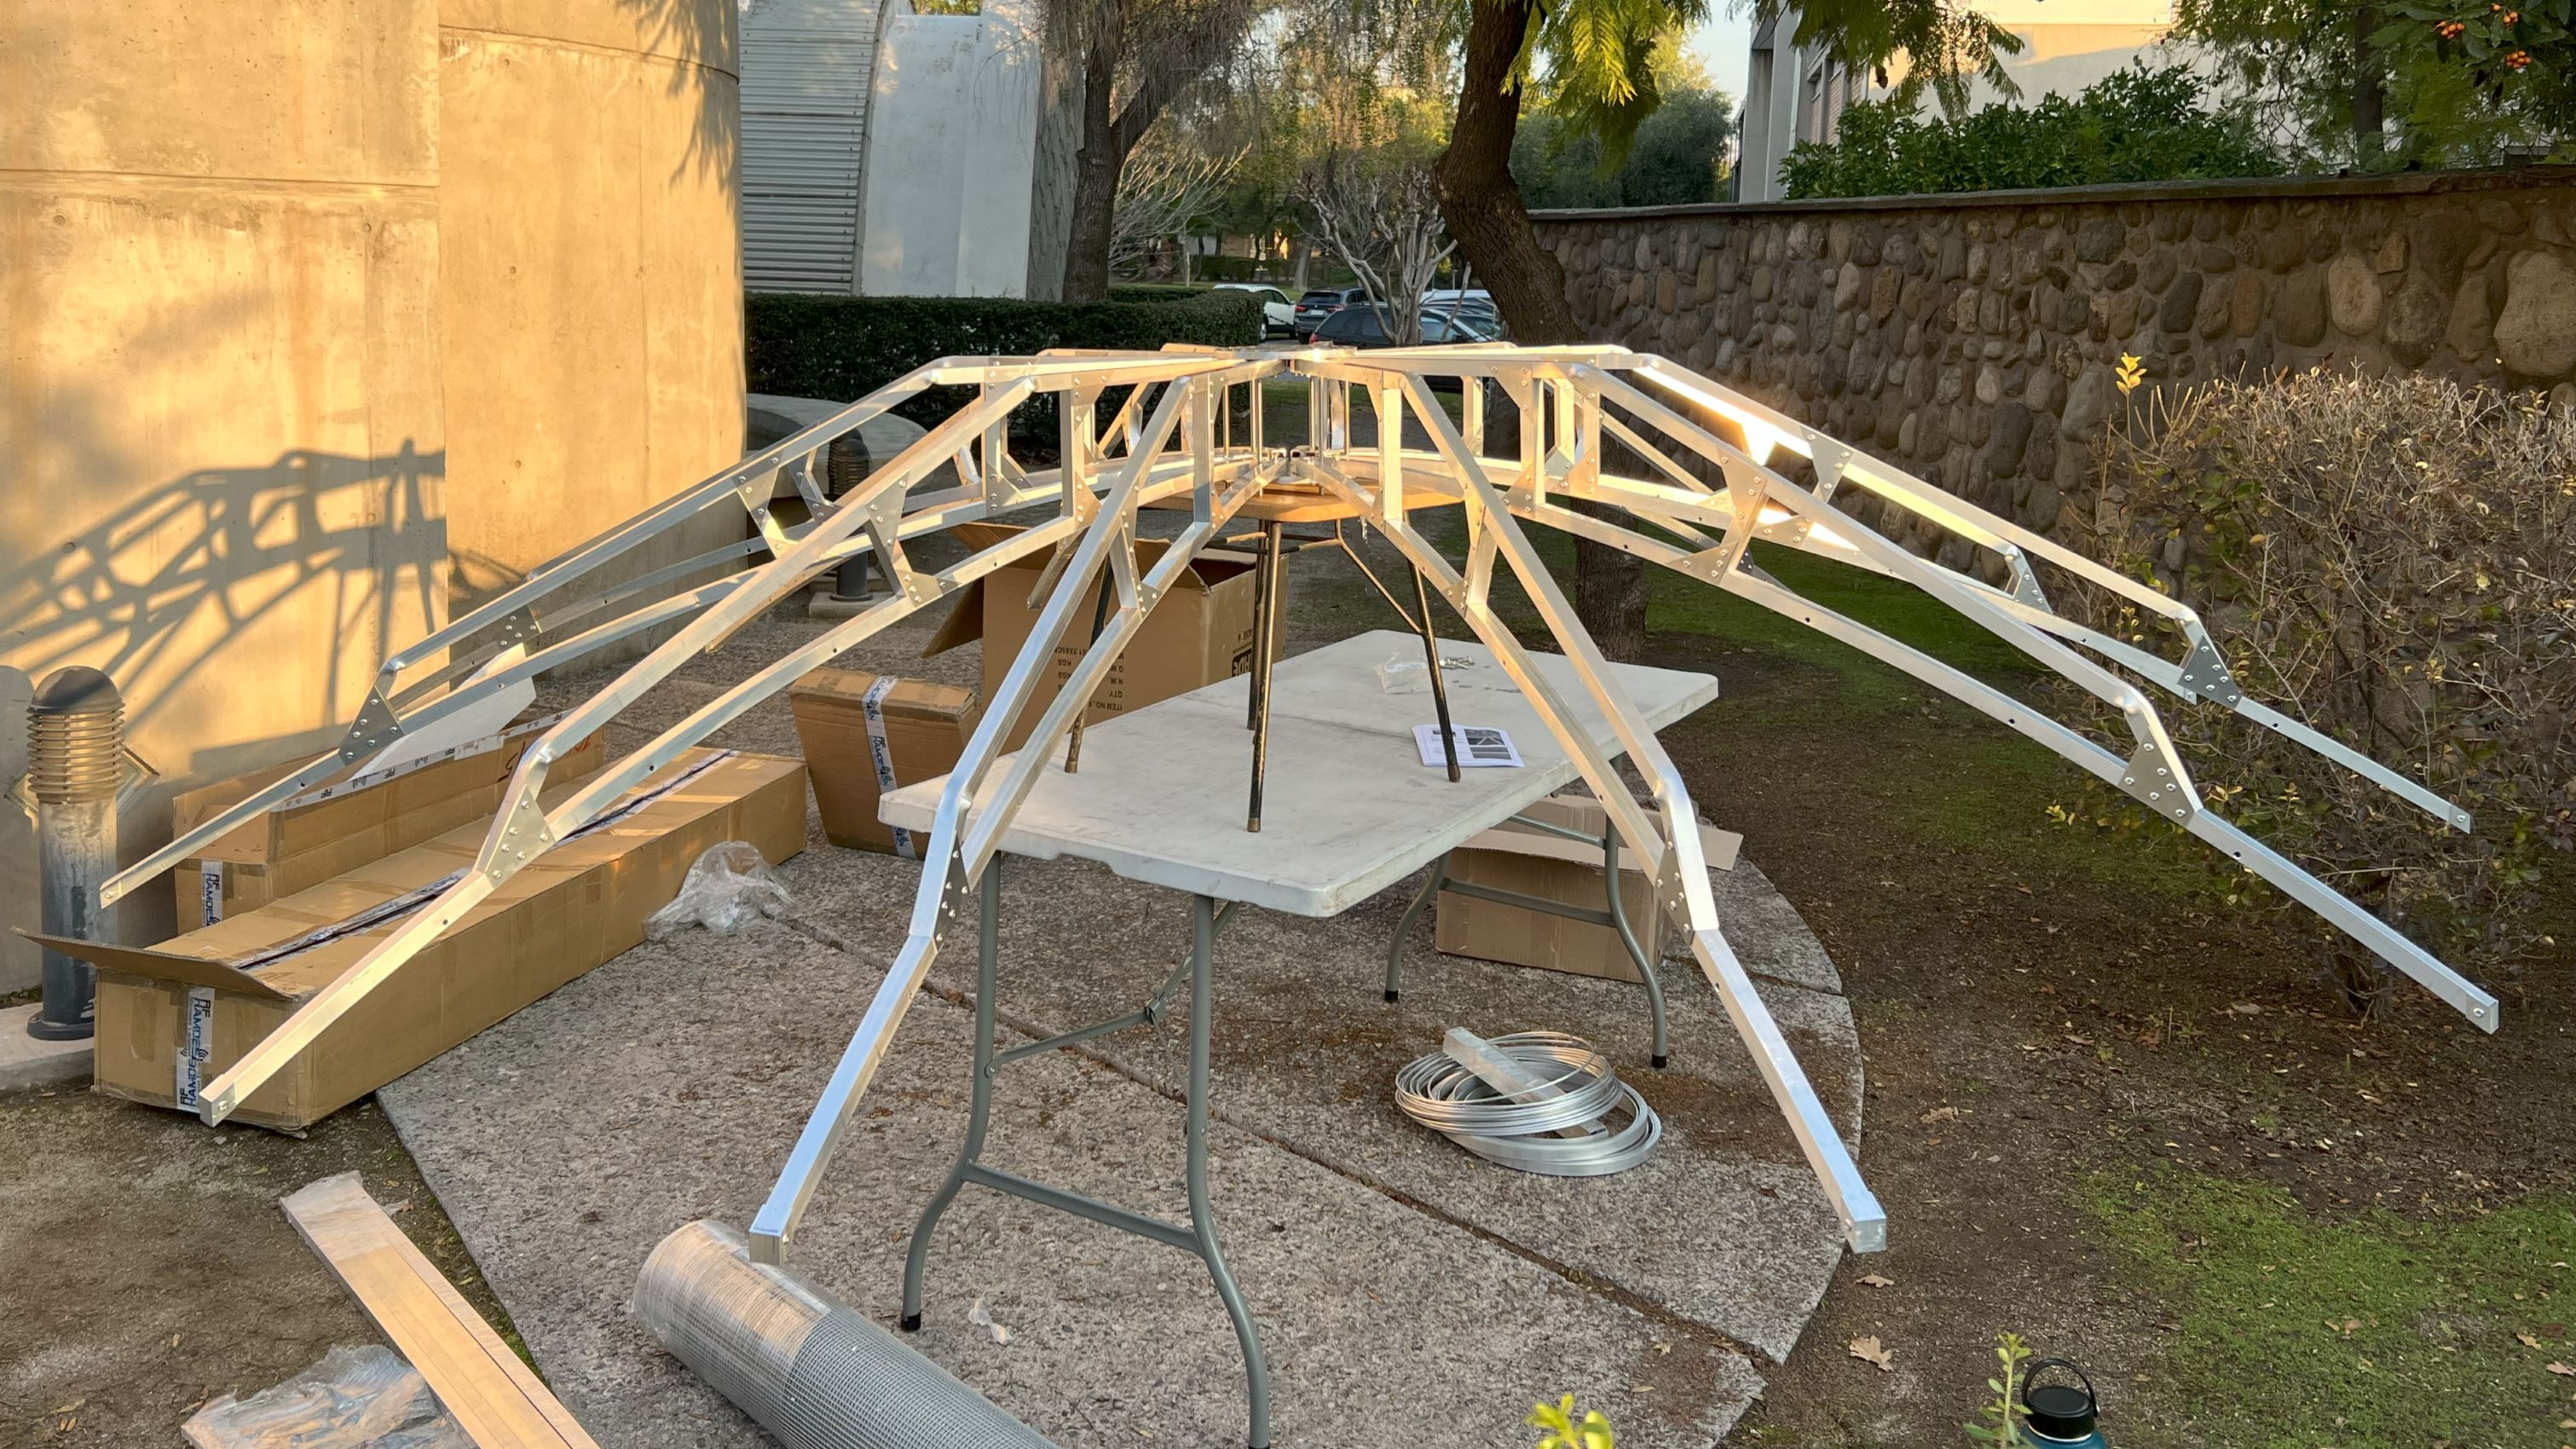
\includegraphics[width=0.8\textwidth]{img/estructura1}
    \caption{Los 12 arcos de alumunio apernados al centro del reflector parabólico.}
    \label{fig:ensamble2}
\end{figure}

En la figura \ref{fig:ensamble2} se pueden ver los 12 arcos de aluminio apernados a los discos de distribucion, que ademas es el punto de anclaje para el soporte de la montura.\\

Luego desenrollan y enderezan los tubos de aluminio que confirmar los anillos donde se tensaeran las mallas metalicas que conforman la superficie del reflector. Con la misma logica se toma la cinta de alumninio, que es aproximadamente de 4 mm de espesor, para enderesarla y prepara las perforaciones para los primeros remaches.\\

\begin{figure}
    \centering
    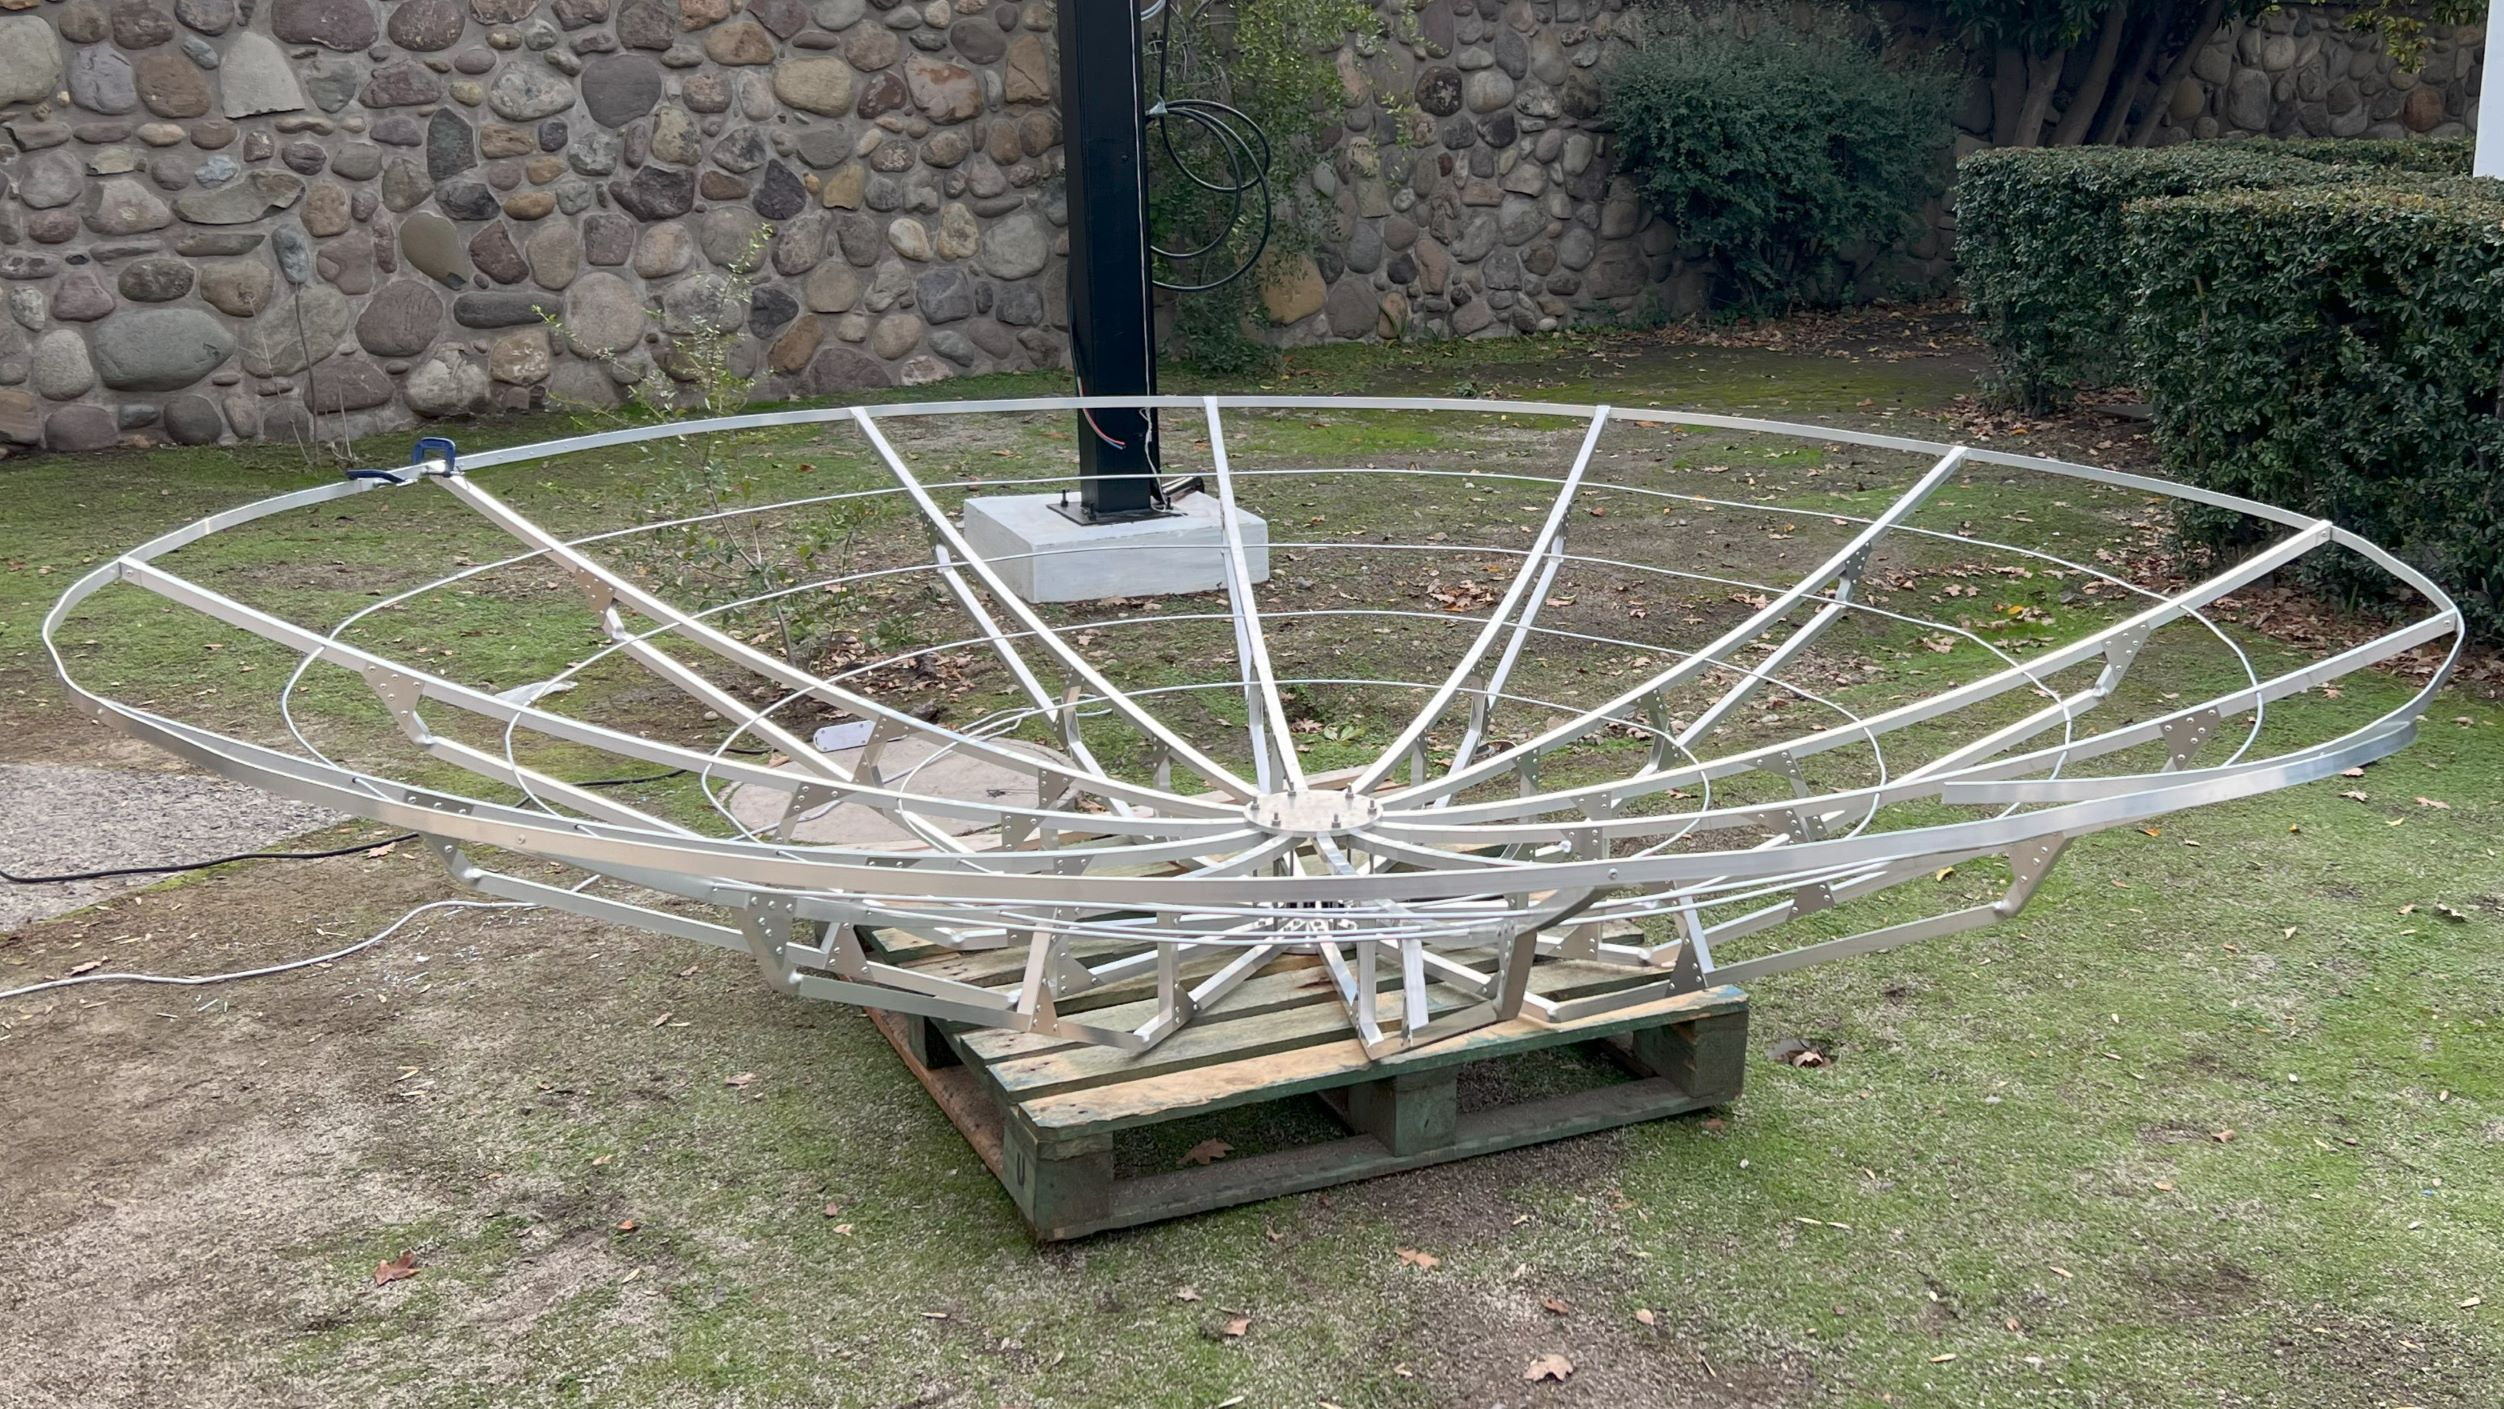
\includegraphics[width=0.8\textwidth]{img/estructura2}
    \caption{Los tubos de aluminio y la cinta de aluminio para la tensión de la malla metálica instalados radialmente en los soportes.}
    \label{fig:ensamble3}
\end{figure}

\subsection{Diseño de soportes adicionales}

Para poder instalar todos los componentes del telescopio, se debian fabricar soportes personalizados y adicionales para así poder utilizar receptores y elementos que no fueran parte del kit original del fabricante. Con el objetivo de reducir los timepos de fabricación y prototipado al usar componentes de aluminio o acero se decidio utilizar impresion 3D con filamento plastico PLA\footnote{Explicacion PLA} de alta resistencia mecanica.\\

Se diseñaron 6 piezas en total con el software de diseño asistido por computadora o \textit{CAD} \textit{Fusion 360} de la compañia \textit{Autodesk}. Todos los comonentes fueron impresos en PLA de alta resistencia o \textit{Hyper-PLA} de la compañia \textit{Creality}, otorgando una mayor resitencia a la flexion de 50\% que el PLA convencional y una elongacion de 6.304\% en comparacion con la del PLA convencional de 3\%. La configuracion de la impresion fue una altura de capa de 0.2 mm, dada por la boquilla utilizada, 4 capas de muralla y un \textit{Infill} o relleno de 60 \%.\\

Una ventaja importante en la elección de la impresion 3D en filamentops plasticos, es su baja incidencia en la deformacion o interferencia del comportamiento de radiofrecuencia, al ser un material no conductor introducido en el campo cercano de los componentes.\\

\begin{figure}
    \centering
    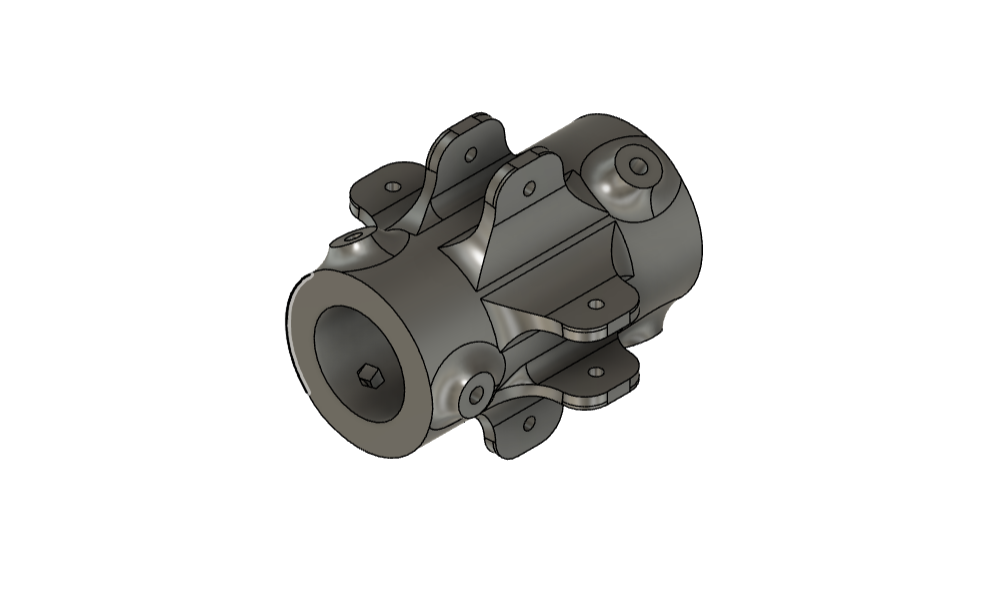
\includegraphics[width=0.8\textwidth]{img/soporte3D5}
    \caption{Union de los doportes de aluminio para el alimentador}
    \label{fig:ensamble4}
\end{figure}

El diseño 3D de la figura \ref{fig:ensamble4} es un soporte que contiene una cabidad centrar cilindrica que conmple la funcion de sostener tanto el alimentador como el receptor por medio de un tubo plastico de PVC\footnote{PVC} que asegura que todo se mantenga alineado con el centro de la parabola, además de permitir un movimiento en el eje de la cabidad cilindrica para ajustar el foco del alimentador.\\

Tiene también 4 ranuras perforadas para aseguirar los soportes con pernos M4 de medida y también 6 perforaciones con cabidades para tuercas M5. Con estas tuercas y con los respectivos tornillos se asegura la poscision del tubo de PVC para fijar el foco una vez encontrado.\\

Las siguientes piezas comparten la misma filosofia de diseño, para poder compatible entre ellas y con el resto de los componentes del telescopio. Además, permiten el rediseño de nuevas piezas para otros alimentadores, cambios de largo en el tubo distriubidor de PVC y en la eleccion de otro material de impreson 3D si se quiciese.\\

\begin{figure}
    \centering
    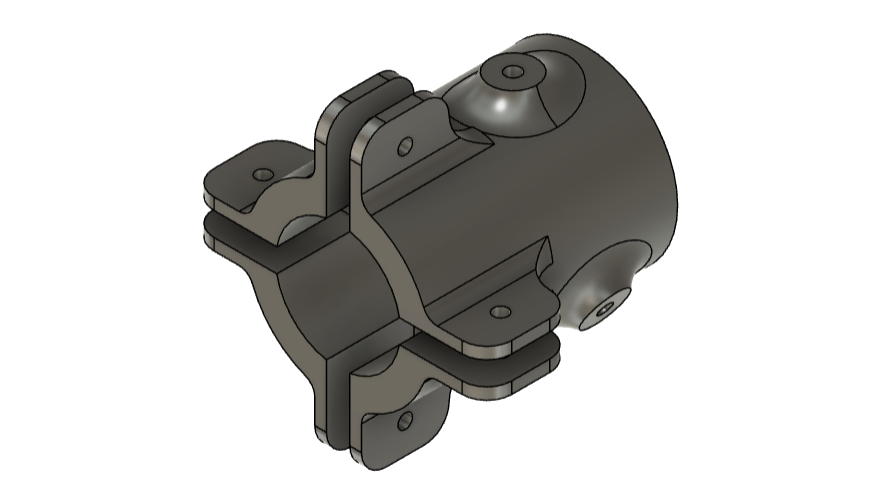
\includegraphics[width=0.8\textwidth]{img/soporte3D1v1}
    \caption{Interfaz de soporte para el tubo de distribucion y otros elementos}
    \label{fig:ensamble5}
\end{figure}

La figura \ref{fig:ensamble5} es un soporte multiproposito que permite acoplar otros soportes de menor complejidad para ser instalados en la zona del alimentador y receptor. Así permite cambios radicales en la instrumentación que se requiera en el futuro sin tener que rediseñar toda la estructura de sujeción.\\

\begin{figure}
    \centering
    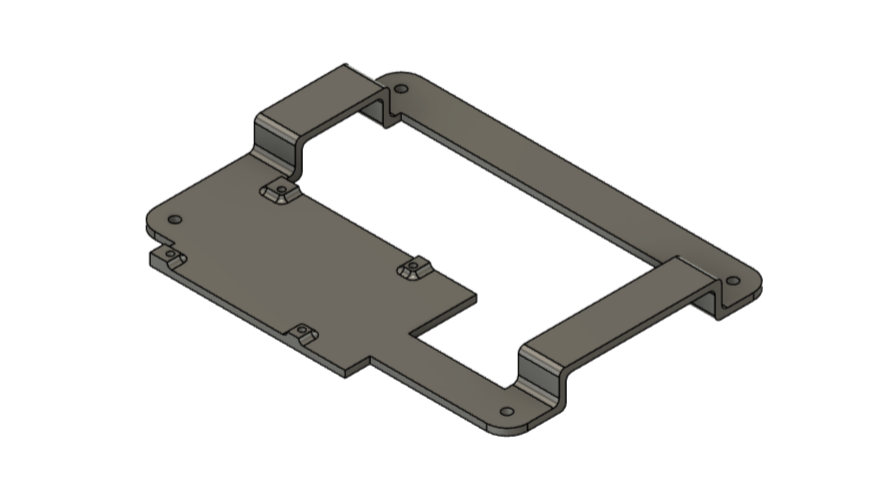
\includegraphics[width=0.8\textwidth]{img/soporte3D7}
    \caption{Soporte interno para electronica de recepción}
    \label{fig:ensamble6}
\end{figure}

El receptor de radiofrecuencia se encuentra dentro de una caja electrica a prueba de agua, pero se requiere un soporte interno para asegurar que la placa de adquisicion de datos y el digitalizador no se muevan y se mantengan en su lugar mientras el telescopio se mueve en distintas elevaciones. La figura \ref{fig:ensamble6} es un soporte que se instala en la caja electrica y permite montar diferentes tipos de receptores y amplificadores.\\

\begin{figure}
    \centering
    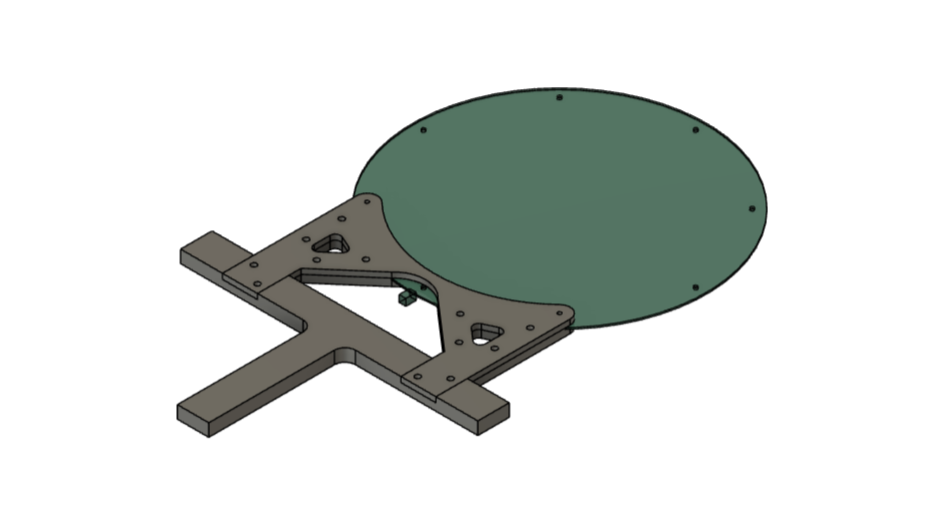
\includegraphics[width=0.8\textwidth]{img/soporte3D4}
    \caption{Soporte para la fuente de calibración de la copa de agua \quotes{estrella artificial}}
    \label{fig:ensamble7}
\end{figure}

La figura \ref{fig:ensamble7} es un soporte que fue diseñdo para instalar la fuente de calibración de la copa de agua o "estrella artificial" en parte superior de la copa de agua del cerro Calan. Se divide en 2 piezas que se unen por medio de pernos M4 de plastico para sujetar la antenna circular por presion y con tronillos pasantes. Ademas para poder asegurar este soporte con faciliada y raídez, se diseño la forma de cruz para que por medio de amarras plasticas se pueda asegurar a la baranda de la copa de agua.\\

\begin{figure}
    \centering
    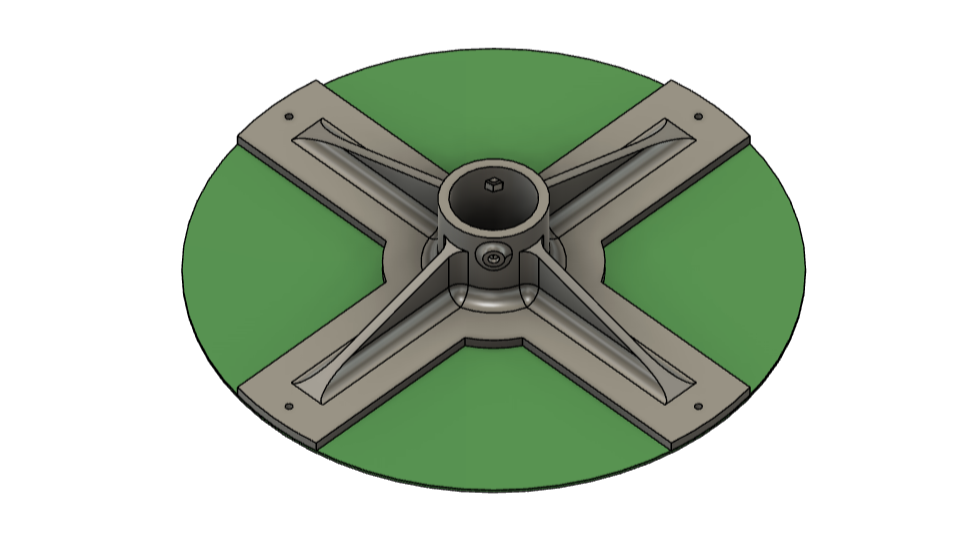
\includegraphics[width=0.8\textwidth]{img/soporte3D2}
    \caption{Soporte para antena circular de alto ancho de banda para cofiguracion de alimentador}
    \label{fig:ensamble8}
\end{figure}

Para las medicones de baja frecuencia (menores a 600 MHz) se debe utilizar la misma antena circular de la figura \ref{fig:ensamble7} pero con un soporte diferente. La figura \ref{fig:ensamble8} es un soporte que permite colocar la antena como alimentador del telescopio por medio del tubo de PVC y asegurarla con pernos M4 al este y pernos plasticos M3 para la antena y el soporte.\\

\begin{figure}
    \centering
    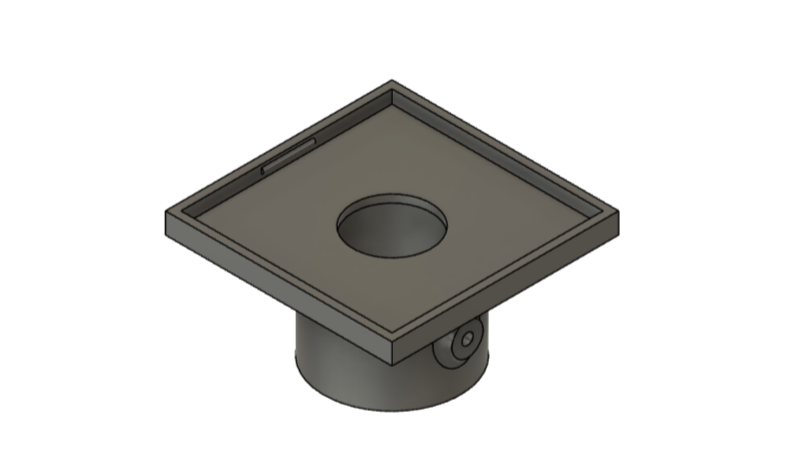
\includegraphics[width=0.8\textwidth]{img/soporte3D6}
    \caption{Soporte para el dipolo exotico como alimentador de 1420MHz}
    \label{fig:ensamble9}
\end{figure}

Al igual que en la figura \ref{fig:ensamble8}, la figura \ref{fig:ensamble9} es un soporte que permite colocar el dipolo exotico como alimentador del telescopio por medio del tubo de PVC. Diferenciandose del sopórte anterior que este diseño permite asegurar la placa de la antena con la deformacion forazada del material impreso, evitando el uso de pernos y tuercas.\\

\subsection{Montura Alt-Azimutal}

El rotor utilizado para la montura alt-azimutal es el modelo \textit{BIG-RAS/HR} de la compañia \textit{RFHamdesign} que esta diseñado para soportar una carga de hasta 319 kg, con una velocidad de movimineto de hasta 2.5 grados por segundo y una resolucion de 0.1 grados para sus encoders.\\

\begin{figure}
    \centering
    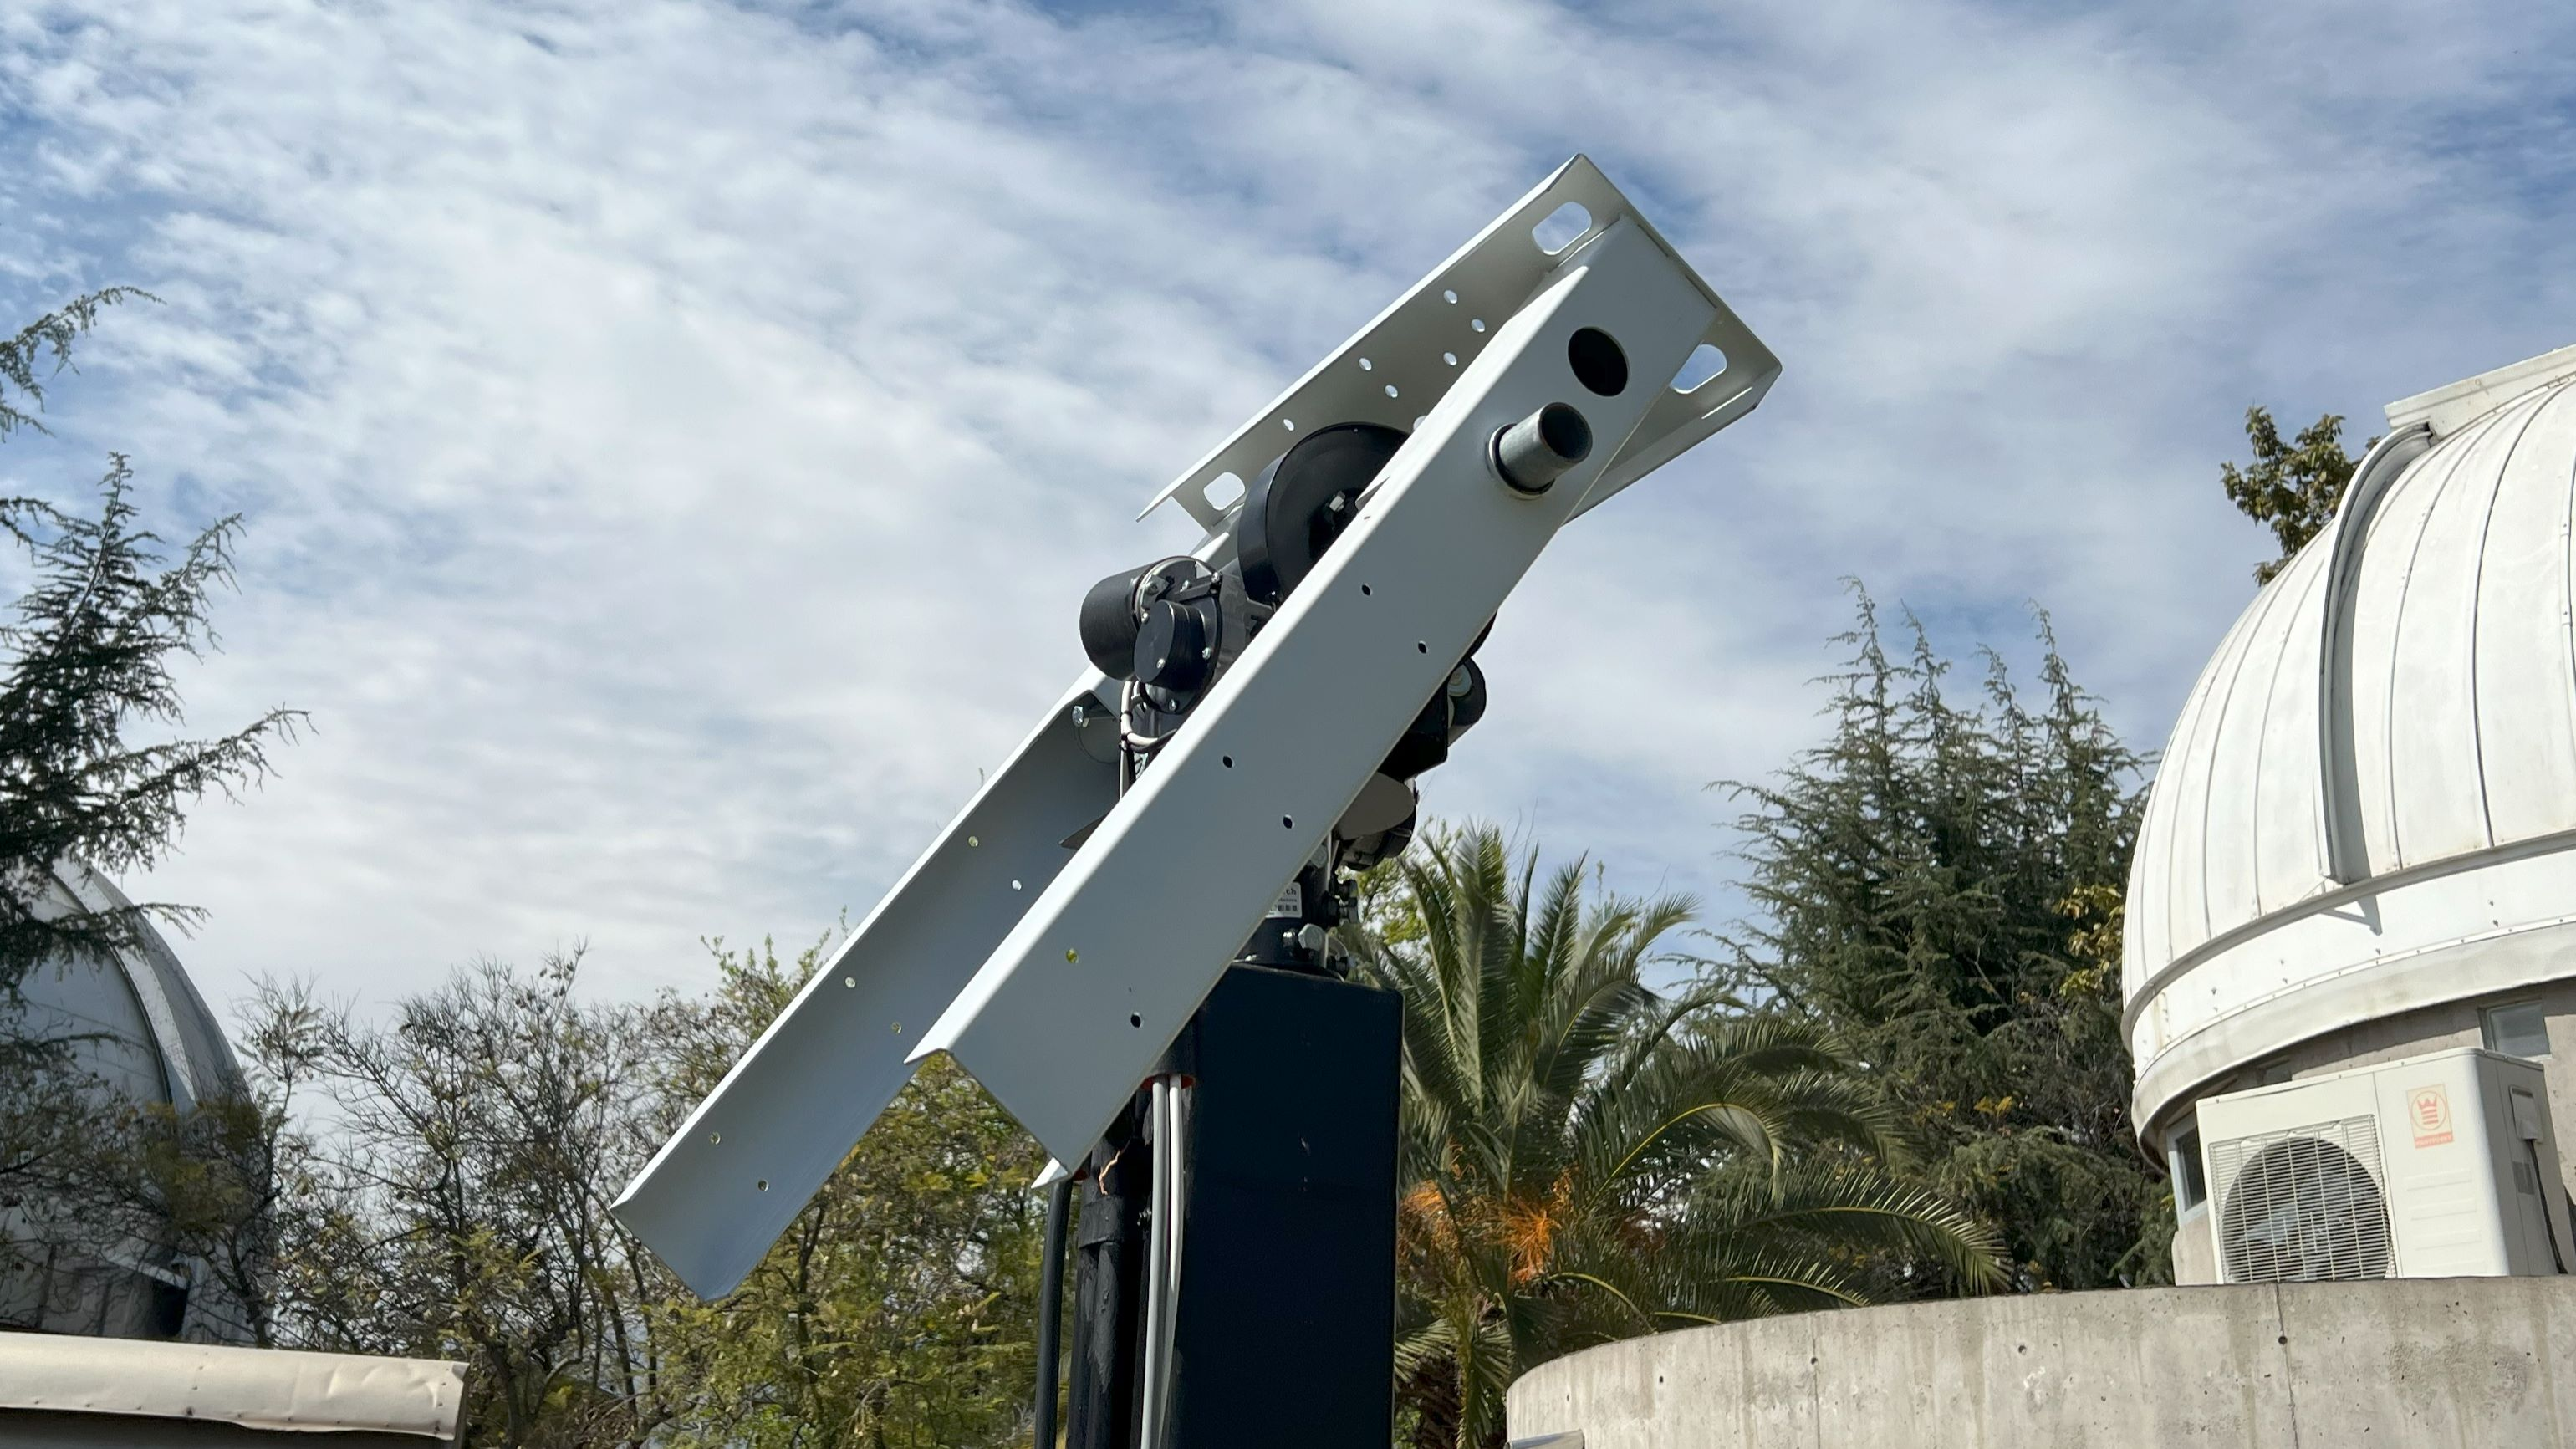
\includegraphics[width=0.8\textwidth]{img/soporte_montura}
    \caption{Rotor \textit{BIG-RAS/HR} de la compañia \textit{RFHamdesign} instalada en el pedestal con la montura de acero.}
    \label{fig:ensamble10}
\end{figure}

En la figura \ref{fig:ensamble10} se puede ver el rotor instalado en el pedestal de acero con la montura que hace la interfaz entre los motores y el reflector. La montura tiene unos brazos traseros perforados para instalar los contrapesos de equilibrio y compensar el torque que ejerce la masa del reflector. La pieza que une la montura con el rotor es una tuberia de acero galbanizado de 46.5 mm de diametro, cortada a la medida de la montura. Todos los pernos de sujecion son M10 de cabeza exagonal.\\

\begin{figure}
    \centering
    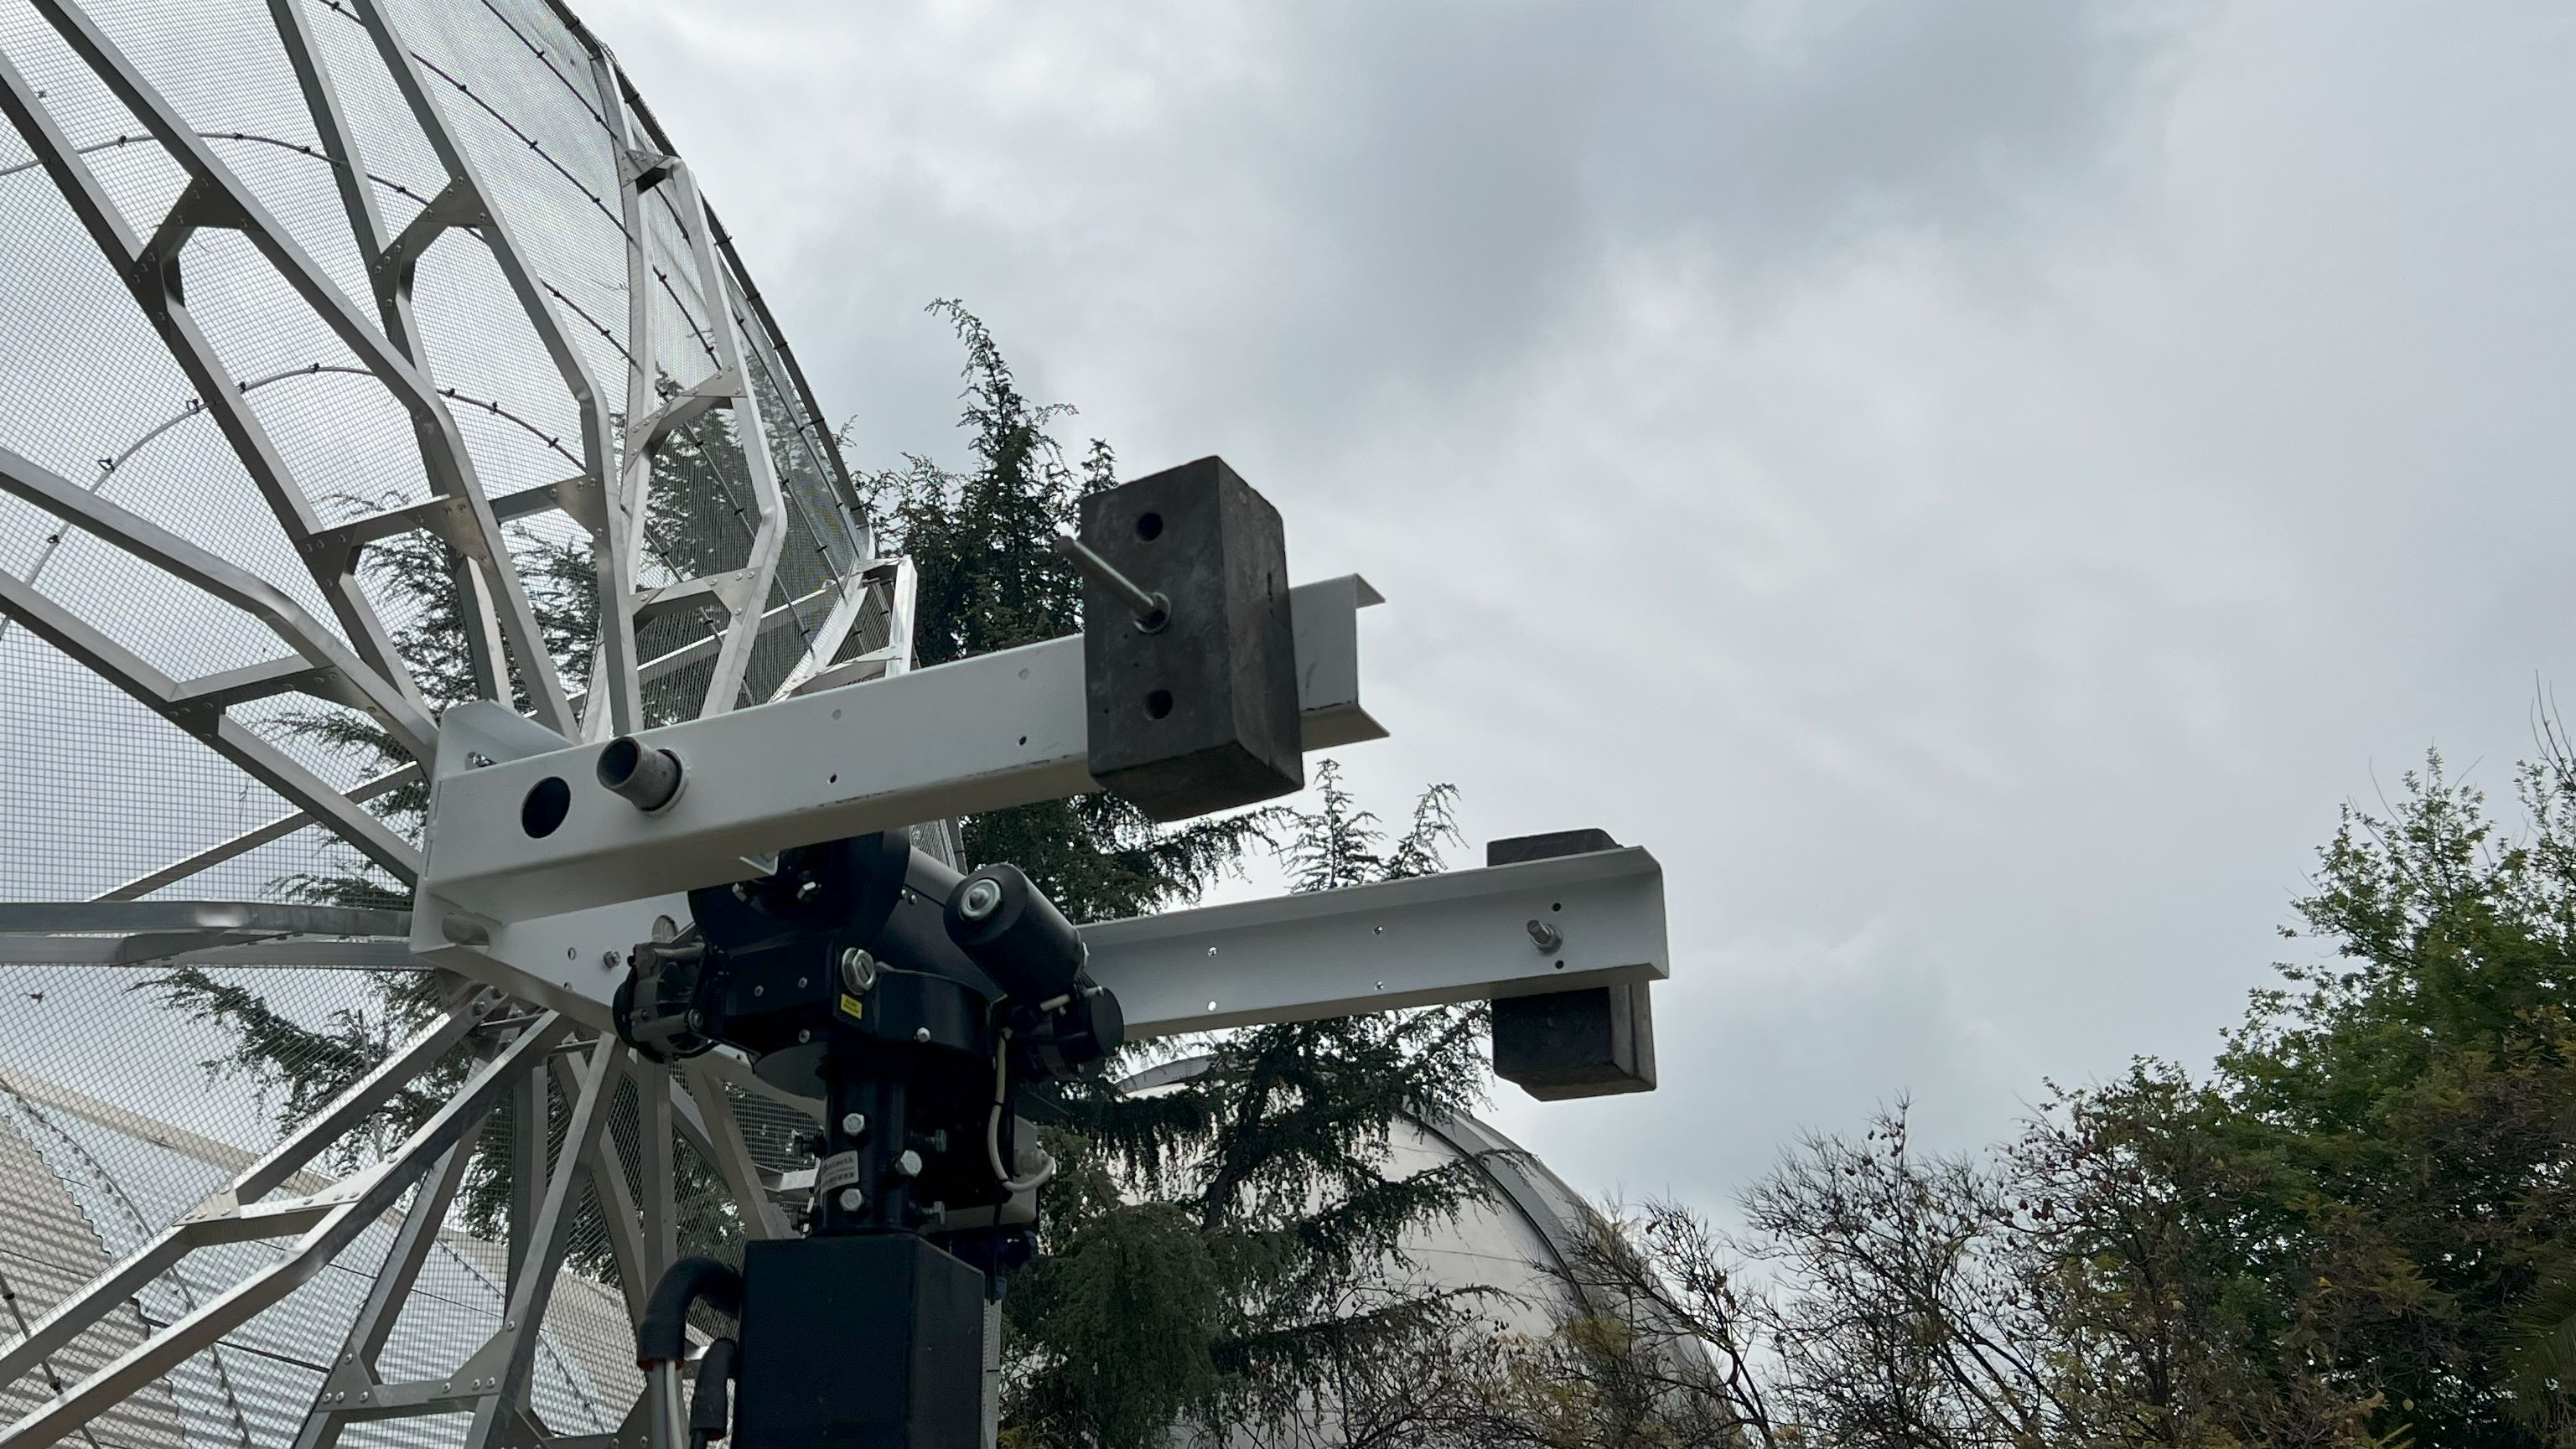
\includegraphics[width=0.8\textwidth]{img/contrapesos}
    \caption{Montura de acero con los contrapesos de equilibrio instalados.}
    \label{fig:ensamble11}
\end{figure}

En la figura \ref{fig:ensamble11} se pueden ver los contrapesos de equilibrio instalados en la montura de acero. Los contrapesos son ladrillos de plomo y cemento de 10 kg cada uno. Se instalaron 4 Ladrillos en total a una distancia de 78 cm de del eje con la tuberia, lugar donde sin ejercer ninguna fuerza sobre la antena o la montura se equilibra con los pernos de sujecion completamente desajustados.\\

La montura es capaz de moverse en 400 grados en azimut y 180 grados en elevacion, con un rango de movimiento de -40 a 360 en los motores horizontales y de 0 a 180 para los motores verticales. Los cuales para mantener rangos de seguridad la motura se mueve entre 0 a 180 grados en azimuth y elevacion, así se minimiza el reisgo de enrrollado de los cables al girar. En la seccion de software se explicará el funcionamiento del algoritmo de movimiento.\\

\subsection{Rack de control}

El rack de control se ecuentra en el edifico más cercano al telescopio, el edifico del meriano, donde tambien se encuentra el telescopio ARTE. El rack consiste en un gabinete de 12 unidades de rack o \textit{U} completamente de acero tanto su cuerpo como la puerta frontal. Con el objetivo de minimizar el RFI que pueda ser introducido por los componentes electronicos, se utilizo un gabinete completamente cerrado y con una puerta frontal de acero conectado a la tierra local.\\


\begin{figure}
    \centering
    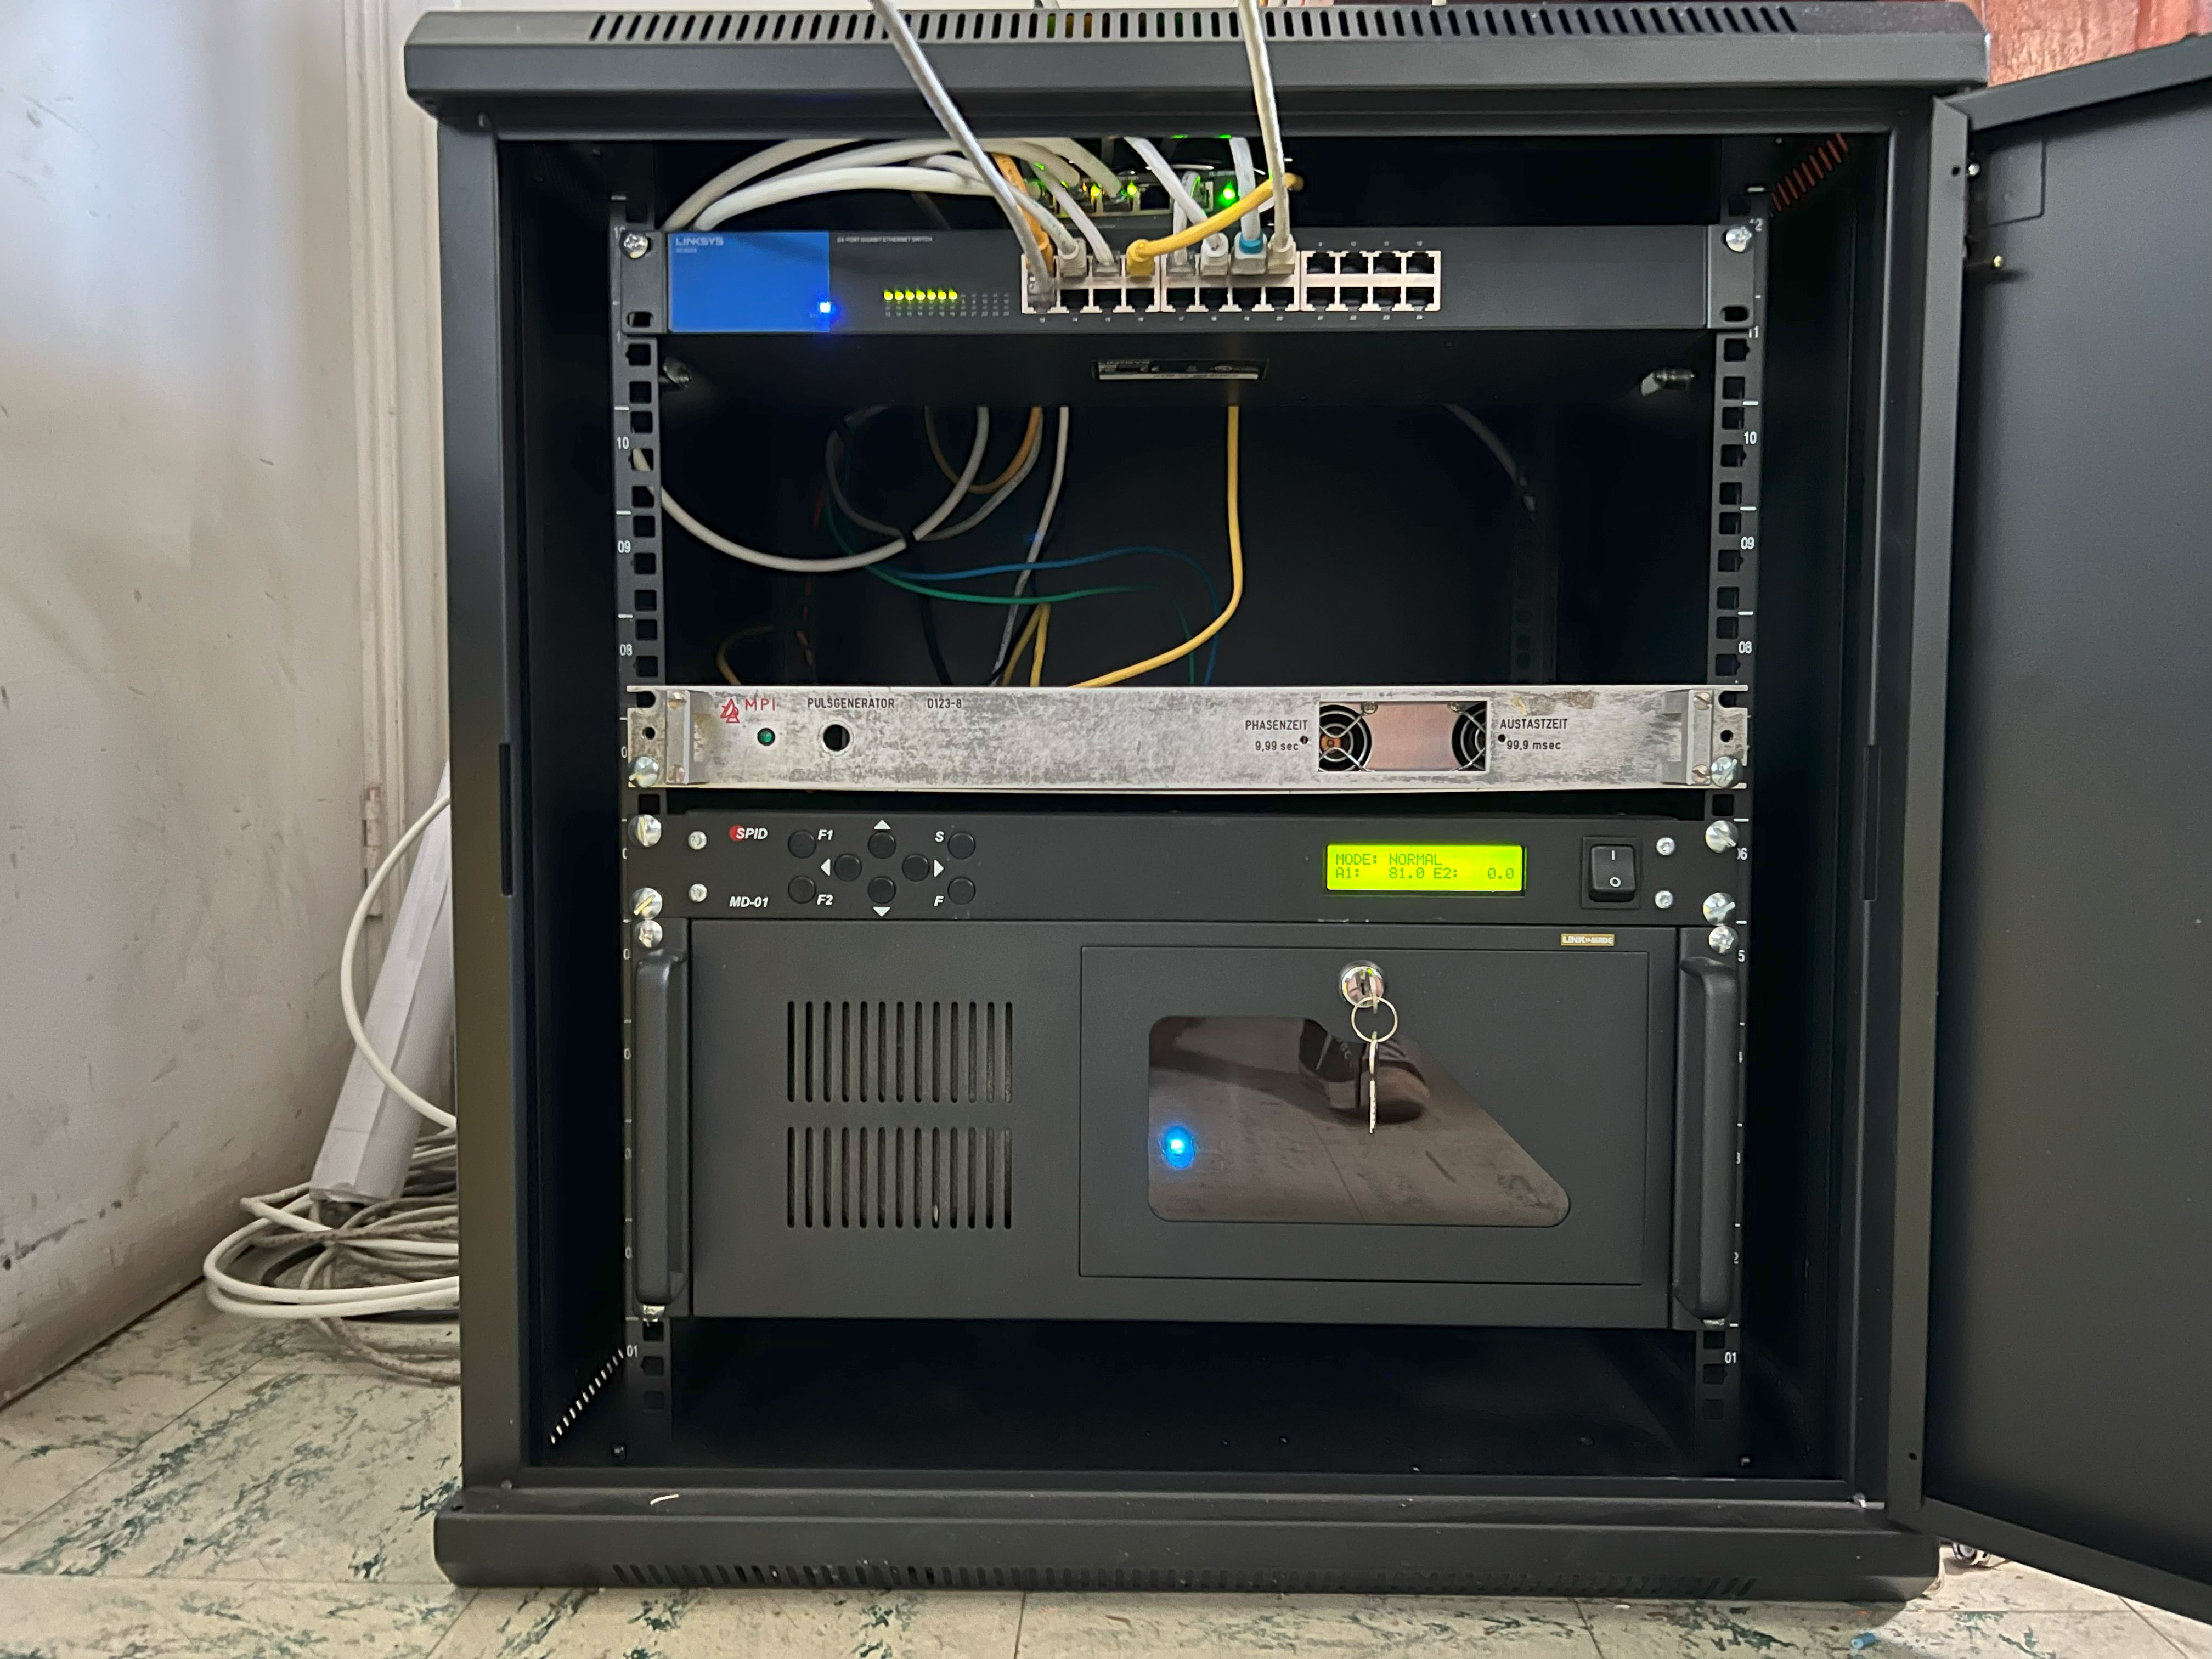
\includegraphics[width=0.8\textwidth]{img/rack}
    \caption{Rack de control con el controlador SPID de la montura y el computador de control.}
    \label{fig:ensamble12}
\end{figure}

En la figura \ref{fig:ensamble12} se puede ver el rack de control con los siguientes elementos ordenados de arriba a abajo: el switch de red, el iyector POE del receptor, la fuente de alimentacion multiple, el controlador de la montura SPID, el computador de control y observacion. Estos elementos se encuentran en la sala de recepcion de ARTE que cuenta con un sistema de climatizacion que mantiene la temperatura a 16 grados celcius constantemente.\\

\section{Alimentador}

Para el alimentador se evaluaron distintas opciones de antenas según su desempeño de ganancia y ancho de banda. Las frecuencias de operacion del telescopio son de 1420 MHz para la banda de hidrógeno y de 300 a 500 MHz para la banda de CHARTS.\\

Como una de las caracteristicas de la cosntruccion del telescopio es la capacidad de intercambiar su alimentador con la estandardizacion de los soportes, se decidio utilizar antenas comerciales que cumplieran con los requerimientos de operacion y se acercaran al rendimiento que declara el fabricante para esta superficie.\\

\subsection{LPDA de alto ancho de banda}

La antena log periodica de dipolo (LPDA) de alto ancho de banda es una antena que se caracteriza por tener una ganancia de 10 dBi y un ancho de banda de 300 a 6000 MHz. Esta antenna se instaló con el elemento más pequeño del arreglo de dipolos en el foco de la parabola. Se orientó verticalmente con respecto al suelo en el telescopio en posicion de azimuth y elevacion de 0 y 0 grados respectivamente.\\

\begin{figure}
    \centering
    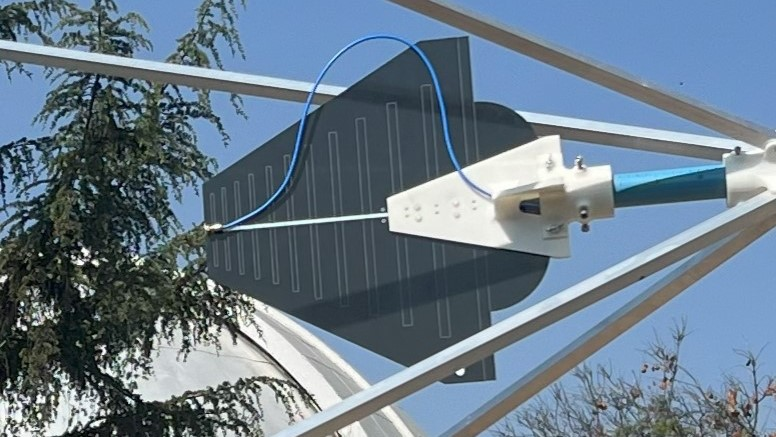
\includegraphics[width=0.8\textwidth]{img/lpda}
    \caption{Antena LPDA de alto ancho de banda instalada en el telescopio.}
    \label{fig:ensamble13}
\end{figure}

La antena de la figura \ref{fig:ensamble13} se instaló en el soporte de la figura \ref{fig:ensamble8} y se conectó al receptor por medio de un cable coaxial de 50 ohmios y 1.5 metros de longitud.\\

\subsection{Dipolo exotico}

El dipolo exotico es una antena que forma el arreglo del telescopio ARTE\cite{Gallardo2023} esta antena se caracteriza por tene una ancho de banda de 400 MHz desde 1000 para el diseño impreso instalado en el telescopio. Esta antenna tiene una ganancia de 3dBi y se ubica en el foco de la parabola a 135 cm del la superficie.\\

\begin{figure}
    \centering
    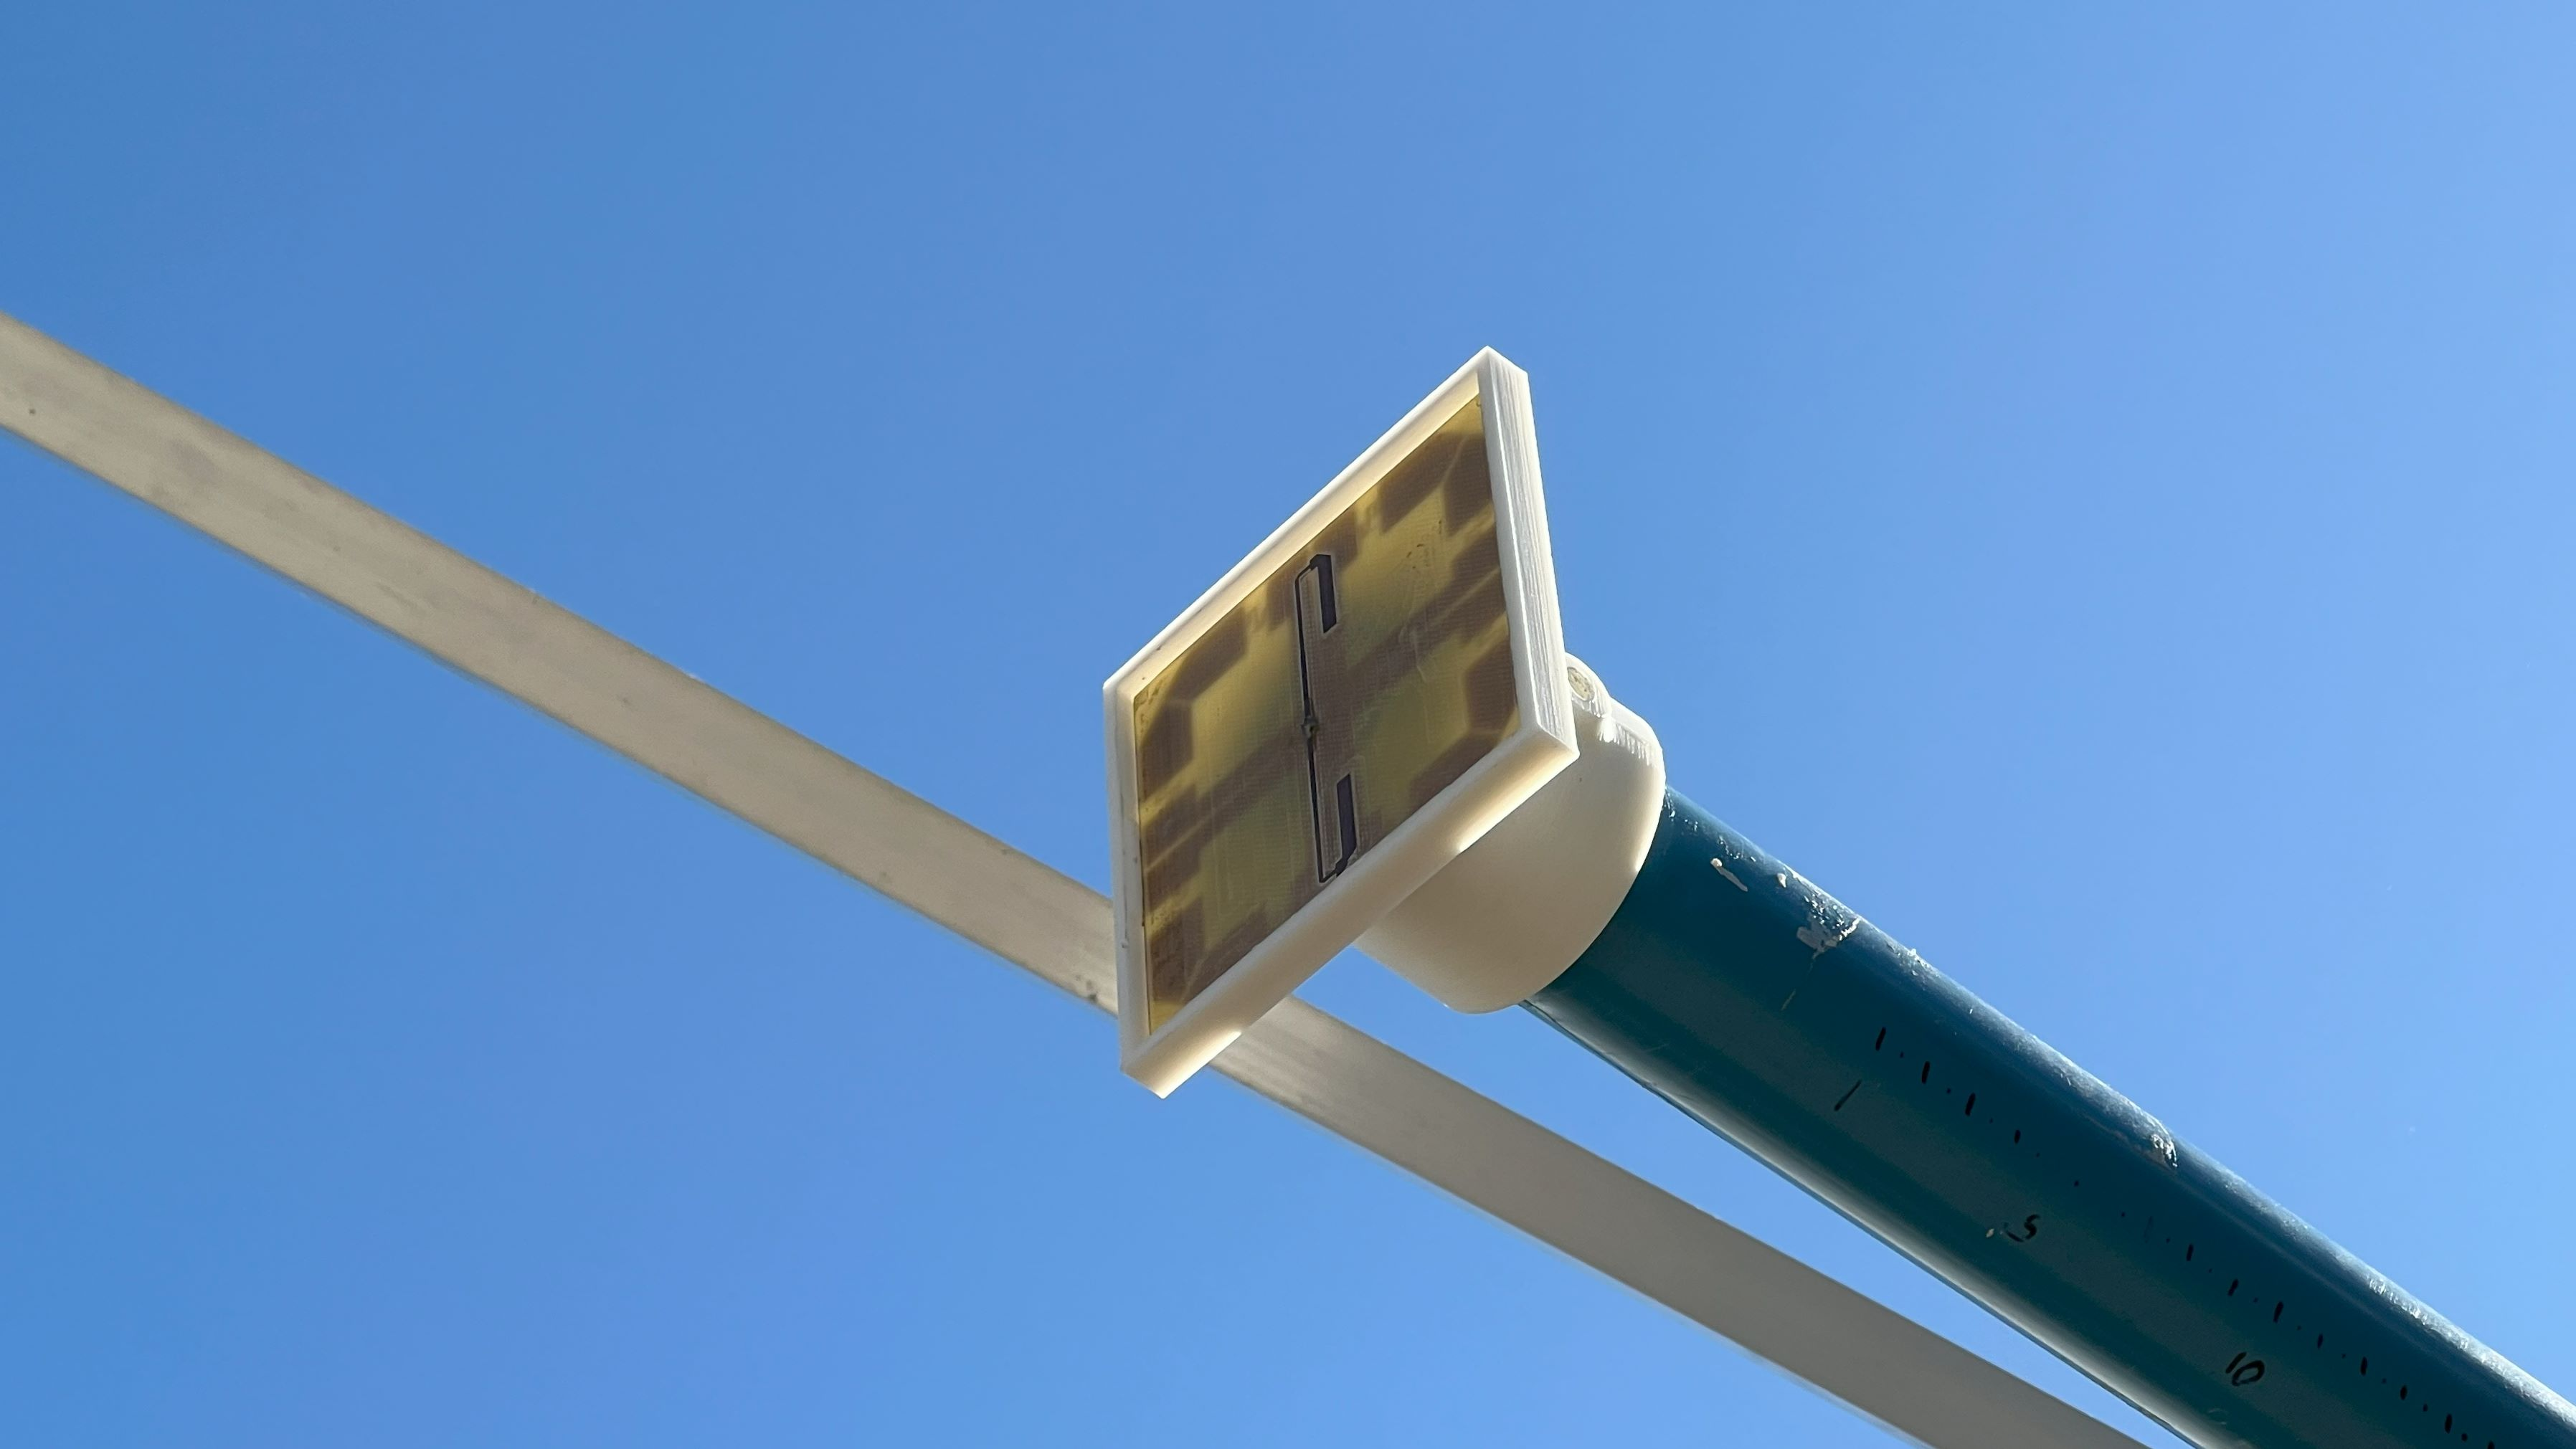
\includegraphics[width=0.8\textwidth]{img/feed}
    \caption{Dipolo de ARTE instalado en el telescopio.}
    \label{fig:ensamble14}
\end{figure}

Esta antena tiene la particularidad de que tiene la ganancia recomendada por el fabricante del reflcetor para utilizar como alimentador a la distancia de 135 cm. Como se puede ver en la figura \ref{fig:ensamble14} la antena de PCB se encuentra instalada en el tubo de PVC con el soporte diseñado de la figura \ref{fig:ensamble9}.\\

\subsection{Antena circular de alto ancho de banda}

Esta antena es la misma que la a utilziar para la fuente de calibracion de la copa de agua, en este caso se quiere utilziar como alimentador en reemplazo de la LPDA de la figura \ref{fig:ensamble13}. Esta antena tiene una ganancia cercana a 3dBi, semejante a la del dipolo de ARTE y lo que se recomienda para el reflector. La antena se instala en el soporte de la figura \ref{fig:ensamble7}.\\

\begin{figure}
    \centering
    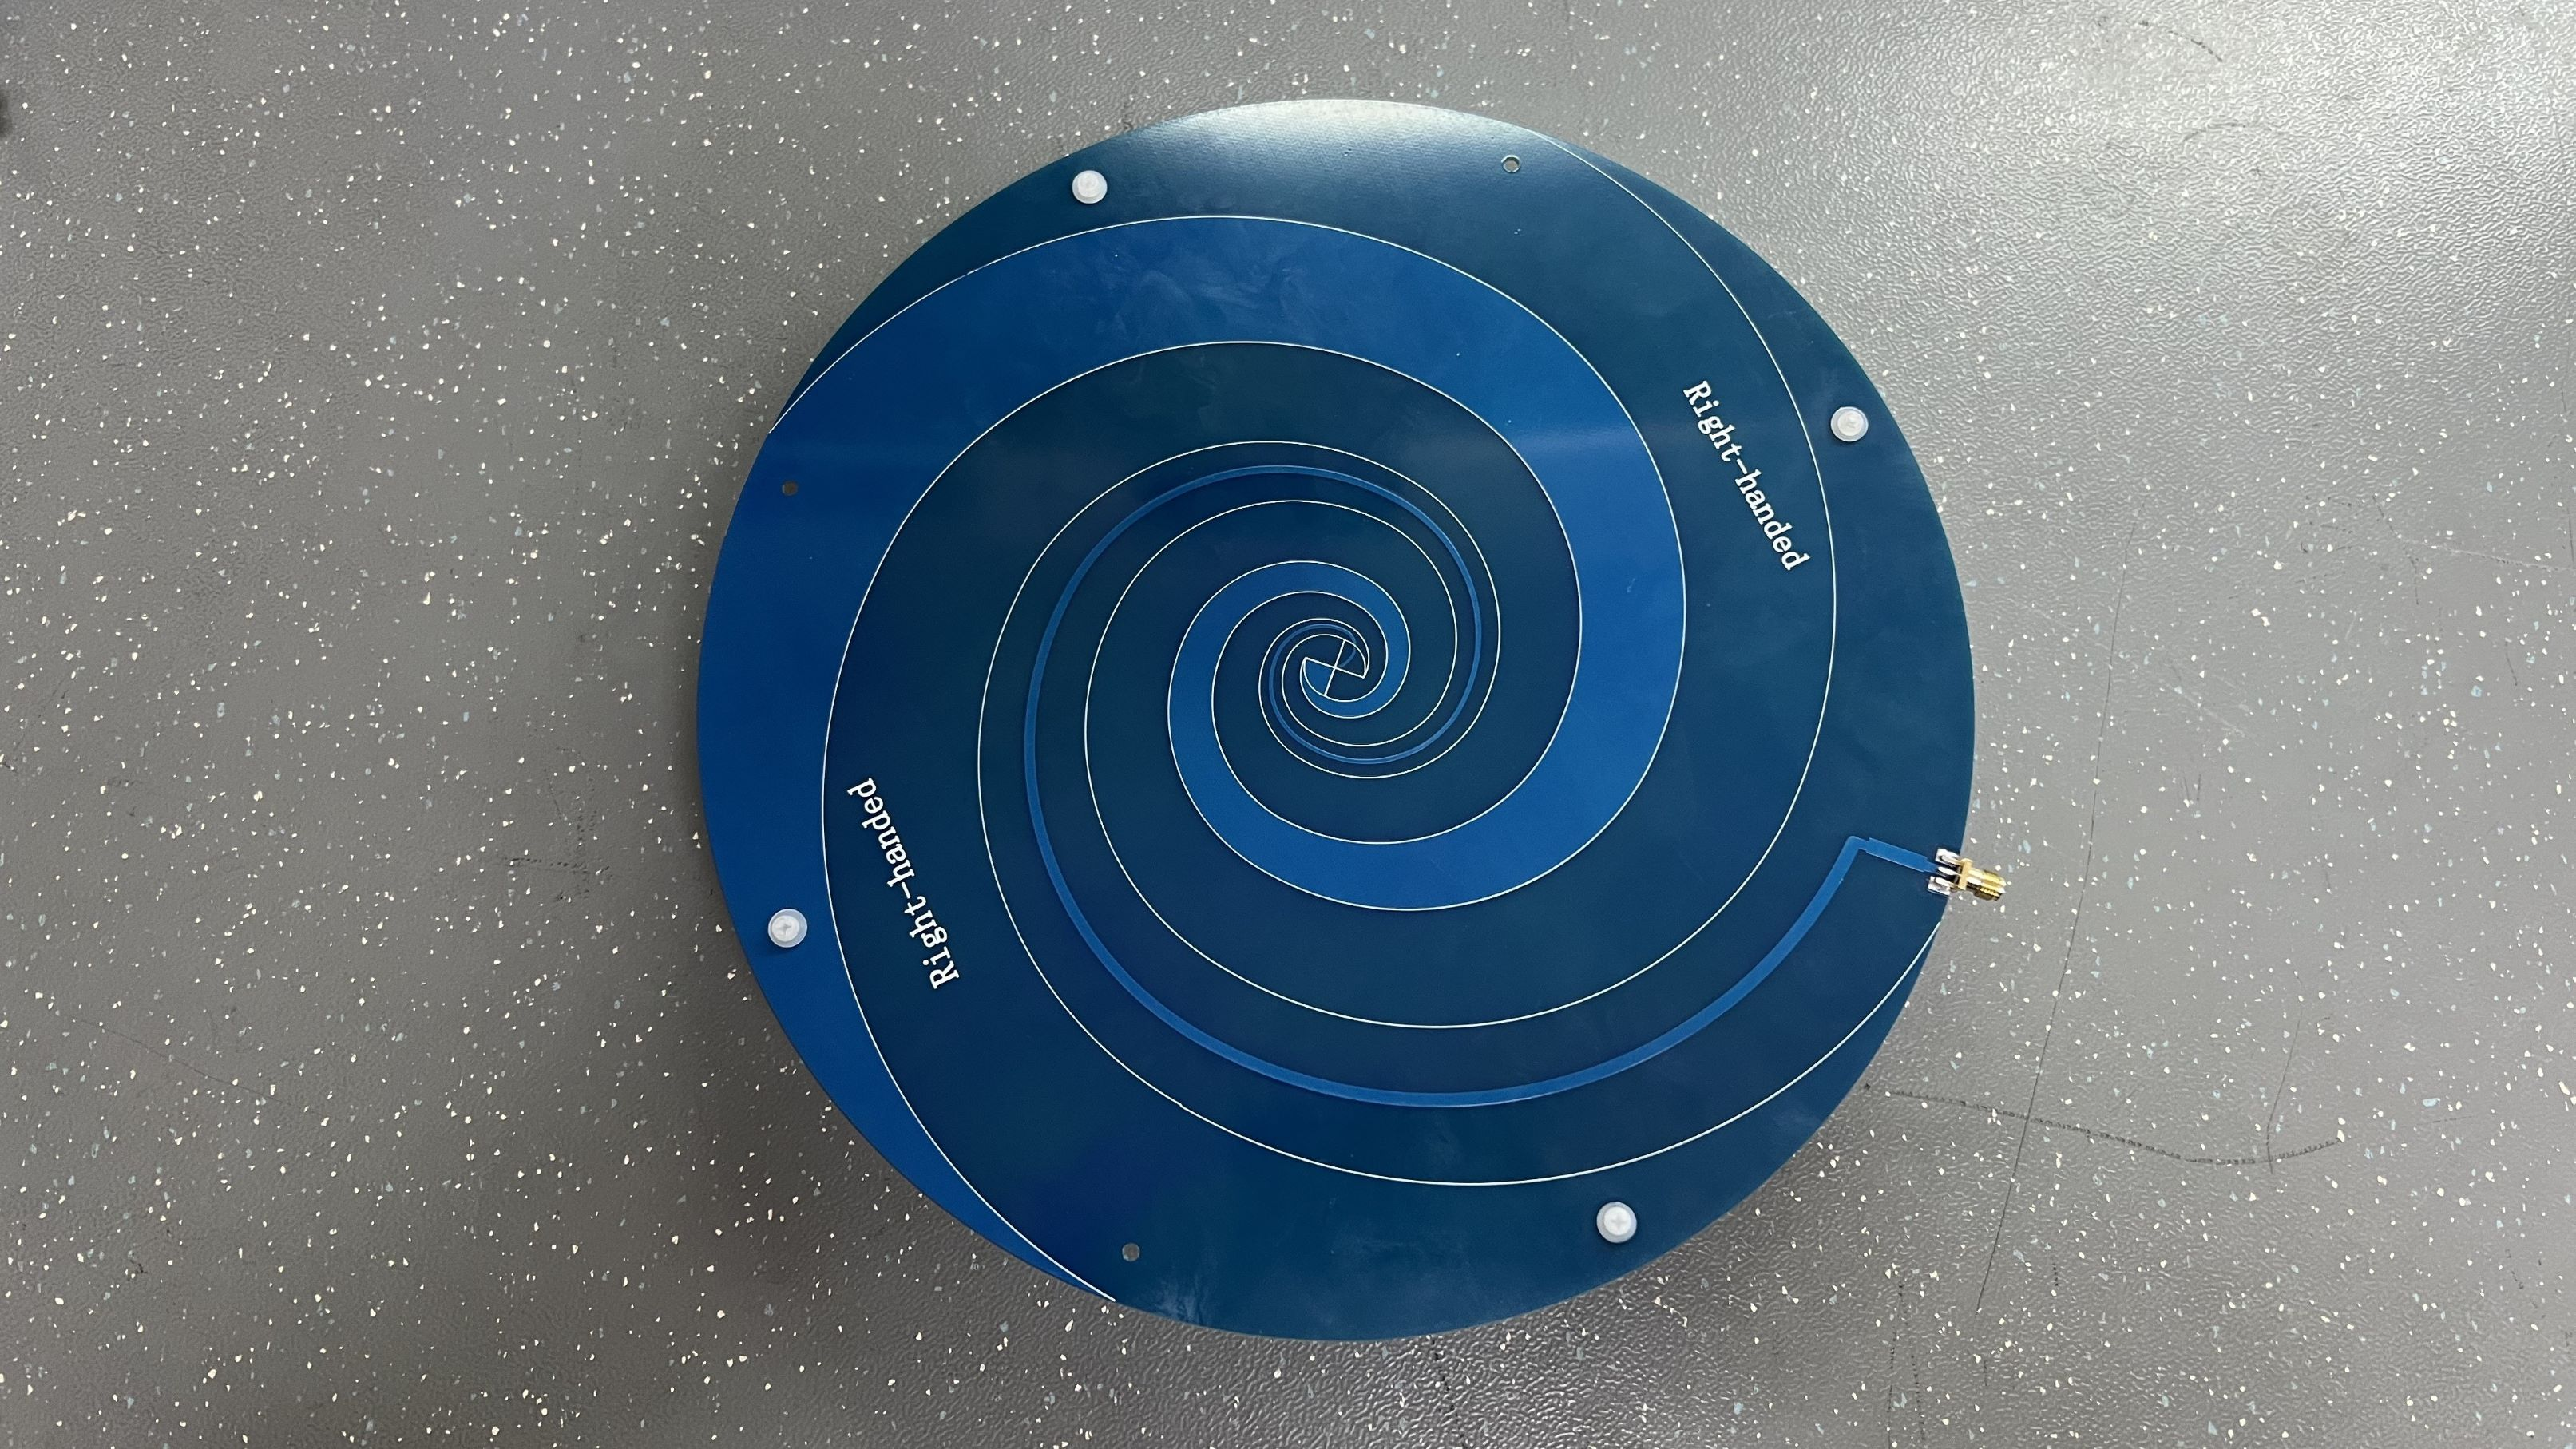
\includegraphics[width=0.8\textwidth]{img/paletaFeed}
    \caption{Antena circular de alto ancho de banda instalada en el telescopio.}
    \label{fig:ensamble15}
\end{figure}


\section{Diseño del receptor}

Para el receptor se optó por utilizar una SDR de bajo costo, una filtro pasabanda optimizado para la observacion de la banda de hidrógeno y un amplificador de bajo ruido. Se tomó en cuenta que estos componentes deben no solo ser de alta precision si no que robustos ya que estaran ubicados lo más cerca posible del alimentador a la interperia.\\

\subsection{Cadena de recepción}

Para la cadena de recpecion cuenta con un empaquetado de un amplificador de bajo ruido de la compañia \textit{Noeelec} que contiene ademas un filtro pasabanda de 75 MHz de ancho de banda centrado en 1420 MHz. El amplificador tiene una ganancia tipica a 1.4 GHz de 35 dB con una figura de ruido de 0.6 dB para la misma frecuencia. Ademas este amplificador puede ser alimentado por bias-tee\footnote{} desde la misma SDR\\

\begin{figure}
    \centering
    
\includegraphics[width=0.8\textwidth]{img/imagen}
    \caption{Amplificador y filtro pasabanda SAWbird H1 de la compañia \textit{Noeelec}.}
    \label{fig:cadena}
\end{figure}

En la figura \ref{fig:cadena} se puede ver el amplificador y filtro pasabanda SAWbird H1 de la compañia conectado a un analizador de espectro y una fuente de ruido para la caracterizacion de la cadena de recepcion.\\

\subsection{Digitalizador y adquisición}

El digitalizador es una RTL-SDR de la oganizacion \textit{RTL-SDR} basado en el chip R820T de \textit{Rafael Micro} que se conecta por USB a un computador para obtener directamente el voltaje complejo de la IF para que sea procesada por el software de adquisicion. Este digitalizador tiene una frecuencia de muestreo maxima de 3.2 MS/s y una resolucion de 8 bits, pero usualmente se utiliza bajo los 2.56 MS/s para que tenga un comportamiento estable\cite{RTLSDR2018}.\\

\begin{figure}
    \centering
    
\includegraphics[width=0.8\textwidth]{img/imagen}
    \caption{RTL-SDR conectada a la cadena de amplificador y una Raspberry PI 4B.}
    \label{fig:digitalizador}
\end{figure}

En la figura \ref{fig:digitalizador} se puede ver la RTL-SDR conectada a la cadena de amplificador y una Raspberry PI 4B con un \textit{Hat} POE. Se utilizo esta configuracion para solo llevar 1 cable ethernet cat 6 por el cual pasaria la energia y los datos. La Raspberry es capaz de alimentar a la SDR que a su vez por medio de su Bias-Tee puede alimentar al amplificador de bajo ruido con la minima cantida posible de cables y conexiones.\\

El cable ethernet utilizado es un cat 6 de 25 metros, que va desde el receptor a el rack de control. Este cable es del tipo FFTP, lo que quiere decir que cada par trensado esta recubierto con una laminade aluminio y a su vez los 4 pares trensados más un conductor de apantallamiento estan recubiertos por otra lamina de alumino que se conecta a tierra en ambos extremos para minimizar el ruido al transportar datos y no producir RFI al telescopio.\\

\section{Software de control y adquisición} \label{sec:software}

La infraestructura digital del telescopio se diseño con un factor principal en mente, que este se pueda operar completamente remoto, por lo que todo el software esta hecho para ser operado desde cualquier lugar con acceso a internet. Accediendo a la terminal de control por medio de SSH\footnote{Secure Shell: } y todos sus sistemas estan conectados a una red local por medio de ethernet.\\

El principal lenguaje de programacion utilizado para el desarrollo de software fue python, por su simplicidad a la hora de generar entornos virtuales de desarrollo y librerias existentes para utilizar los diversos subsistemas, como por ejemplo, el uso de la libreria de \textit{astropy} para los calculos de seguimiento.\\

\subsection{Control de la montura}

El controlador del rotor requiere una comunicacion especifica en hexagesimal para moverse y a travez del mismo protocolo responde con la posicion en la cual se encuentra. Para esto se creó una libreria en python basada en el protocolo Rot2Prog\cite{Rot2Prog} que empaqueta y traduce los comandos de movimiento, elevacion y azimut. Esta libreria es un archivo de python por el nombre de spid.py, la que es importada para todos los demas codigos de control.\\

\paragraph{control.py} es el codigo principal de control, tiene la capacidad de mandar una posicion de azimuth y elevacion, de pedir la posicion actual de la montura, de reiniciar el controlodor en caso que no responda a los comandos y una de las funciones más importantes el parado de emergencia de cualquier movimiento.\\

\paragraph{cpt\_traking\_software.py} Este es un software más sofisticado que se creo para el seguimiento de cuerpos celestes. a partir de las coordenadas de declinacion y ascencion recta, el software calcula la posicion de la montura para este astro segun la ubicacion del telescopio y la hora local.\\

\begin{figure}
    \centering
    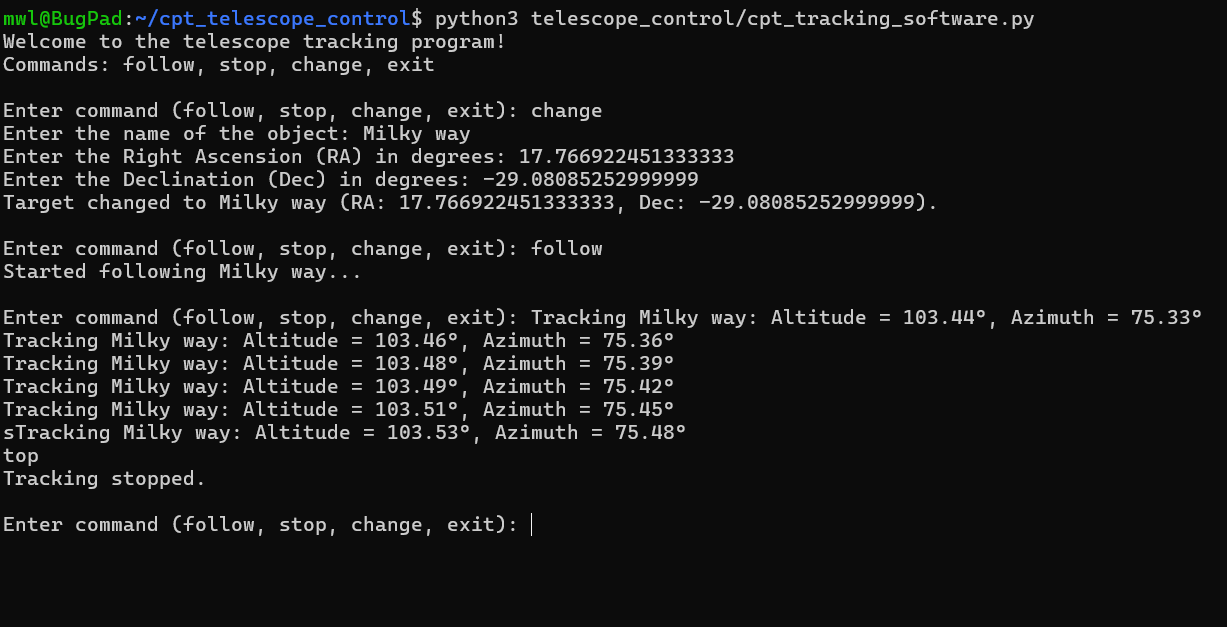
\includegraphics[width=0.8\textwidth]{img/traking}
    \caption{cpt\_traking\_software.py en funcionamiento.}
    \label{fig:control}
\end{figure}

En la figura \ref{fig:control} se puede ver el software en funcionamiento, con las opciones de cambiar el objeto a seguir \textit{change}, el seguimiento del objeto \textit{follow} y el parado del movimiento\textit{stop}. El software es capaz de invertir la posicion de elevacion del telescopio para minimizar el movimiento en azimut y evitar que los cables puedan enrollarse entre si.\\

Por ejemplo si al calcular que la posicion del astro en elevacion de 50 grados y azimuth de 315, requiere un movimiento de más de 180 grados en azimut, el software invierte la posicion de elevacion para que el movimiento sea menor a 180 grados resultando en que el telescopio apunte a 130 grados de elevacion y a 135 grados en azimut. De forma automatica, si el astro tiene una elevacion menor a los 30 grados, o mayor a 150 grados en la inversion, este deja de seguir el astro ya que a esta elevacion la interferencia de radio es muy notoria en las observaciones por efectos atmosfericos y cada vez entra en la linea de vista elementos de comunicaciones inhalambricas terrestres.\\

\subsection{Adquisición de datos} 

Para la adquisicion de datos se crearon 2 softwares en python para esta tarea, una para adquirir una acumulacion de espectros para las observaciones de un objeto celeste y otro para la calibracion del instrumento.\\

\paragraph{rtl\_spectra.py} Es un script que utiliza la radio RTL-SDR para obtener espectros mediante un comando de especifico, este se utiliza principalmente para las caracterizaciones y las mediciones. Este se utiliza en conjunto con el software de control para crear las variantes de medicion de patro de radiacion. Se puede configurar la taza de datos, el tamaño de la FFT, la cantidad de espectros tomados y el formato de guardado.\\

\paragraph{cpt\_rtl\_adquisition.py} Es el software de observacion, el cual tiene un \textit{Ring buffer} o un acumulador de espectros flotantes, esto quiere decir que, segun como se configure, puede acumular una cantidad de espectros que se van actualizand constantemente con nuevos y eliminando los viejos en la ventana de tiempo que se requiera o en lo que la memoria pueda guardar.\\

Al igual que el script anterior este se puede configurar para la taza de datos, el tamaño de la FFT, la cantidad de espectros tomados y el formato de guardado. Este, por otra parte, esta diseñado para obtener una gran cantidad de espectros para ser guardados en una estructura eficiente en espacio en codigo binario. Tambien tiene la tarea de mostrar en tiempo real la acumulacion promediada de los espectros y en paralelo obtener las muestras y agregarlas al ring-buffer.\\


\section{Infraestructura de caracterizacion}

Para caracterizar el telescopio se requieren de una serie de instrumentos y elementos que permitan obtener los datos necesarios para la calibracion y la verificacion de los resultados obtenidos.\\

\subsection{Fuente de calibración}

Ya que el campo lejano de las antenas electricamente grandes, como es el caso de una antena de apertura. Para medir el patron de radiacion en potencia de una antena se requiere de una fuente de radiofrecuencia conocida a una distancia mayor a la de campo lejao de la antena que se quiere medir.\\

Para esto se instaló una antena de alto ancho de banda (192 MHz a 8 GHz) en la copa de agua del cerro calan, con un cable coaxial de 20 metros de longitud. Puediendo así dejar la anetna instalada en la parte superior y poder conectar generadores de señales desde la parte inferior. Esta antena le llamaremos la \quotes{estrella artificial}.\\

\begin{figure}[h!]
    \centering
    \begin{subfigure}{0.45\textwidth}
        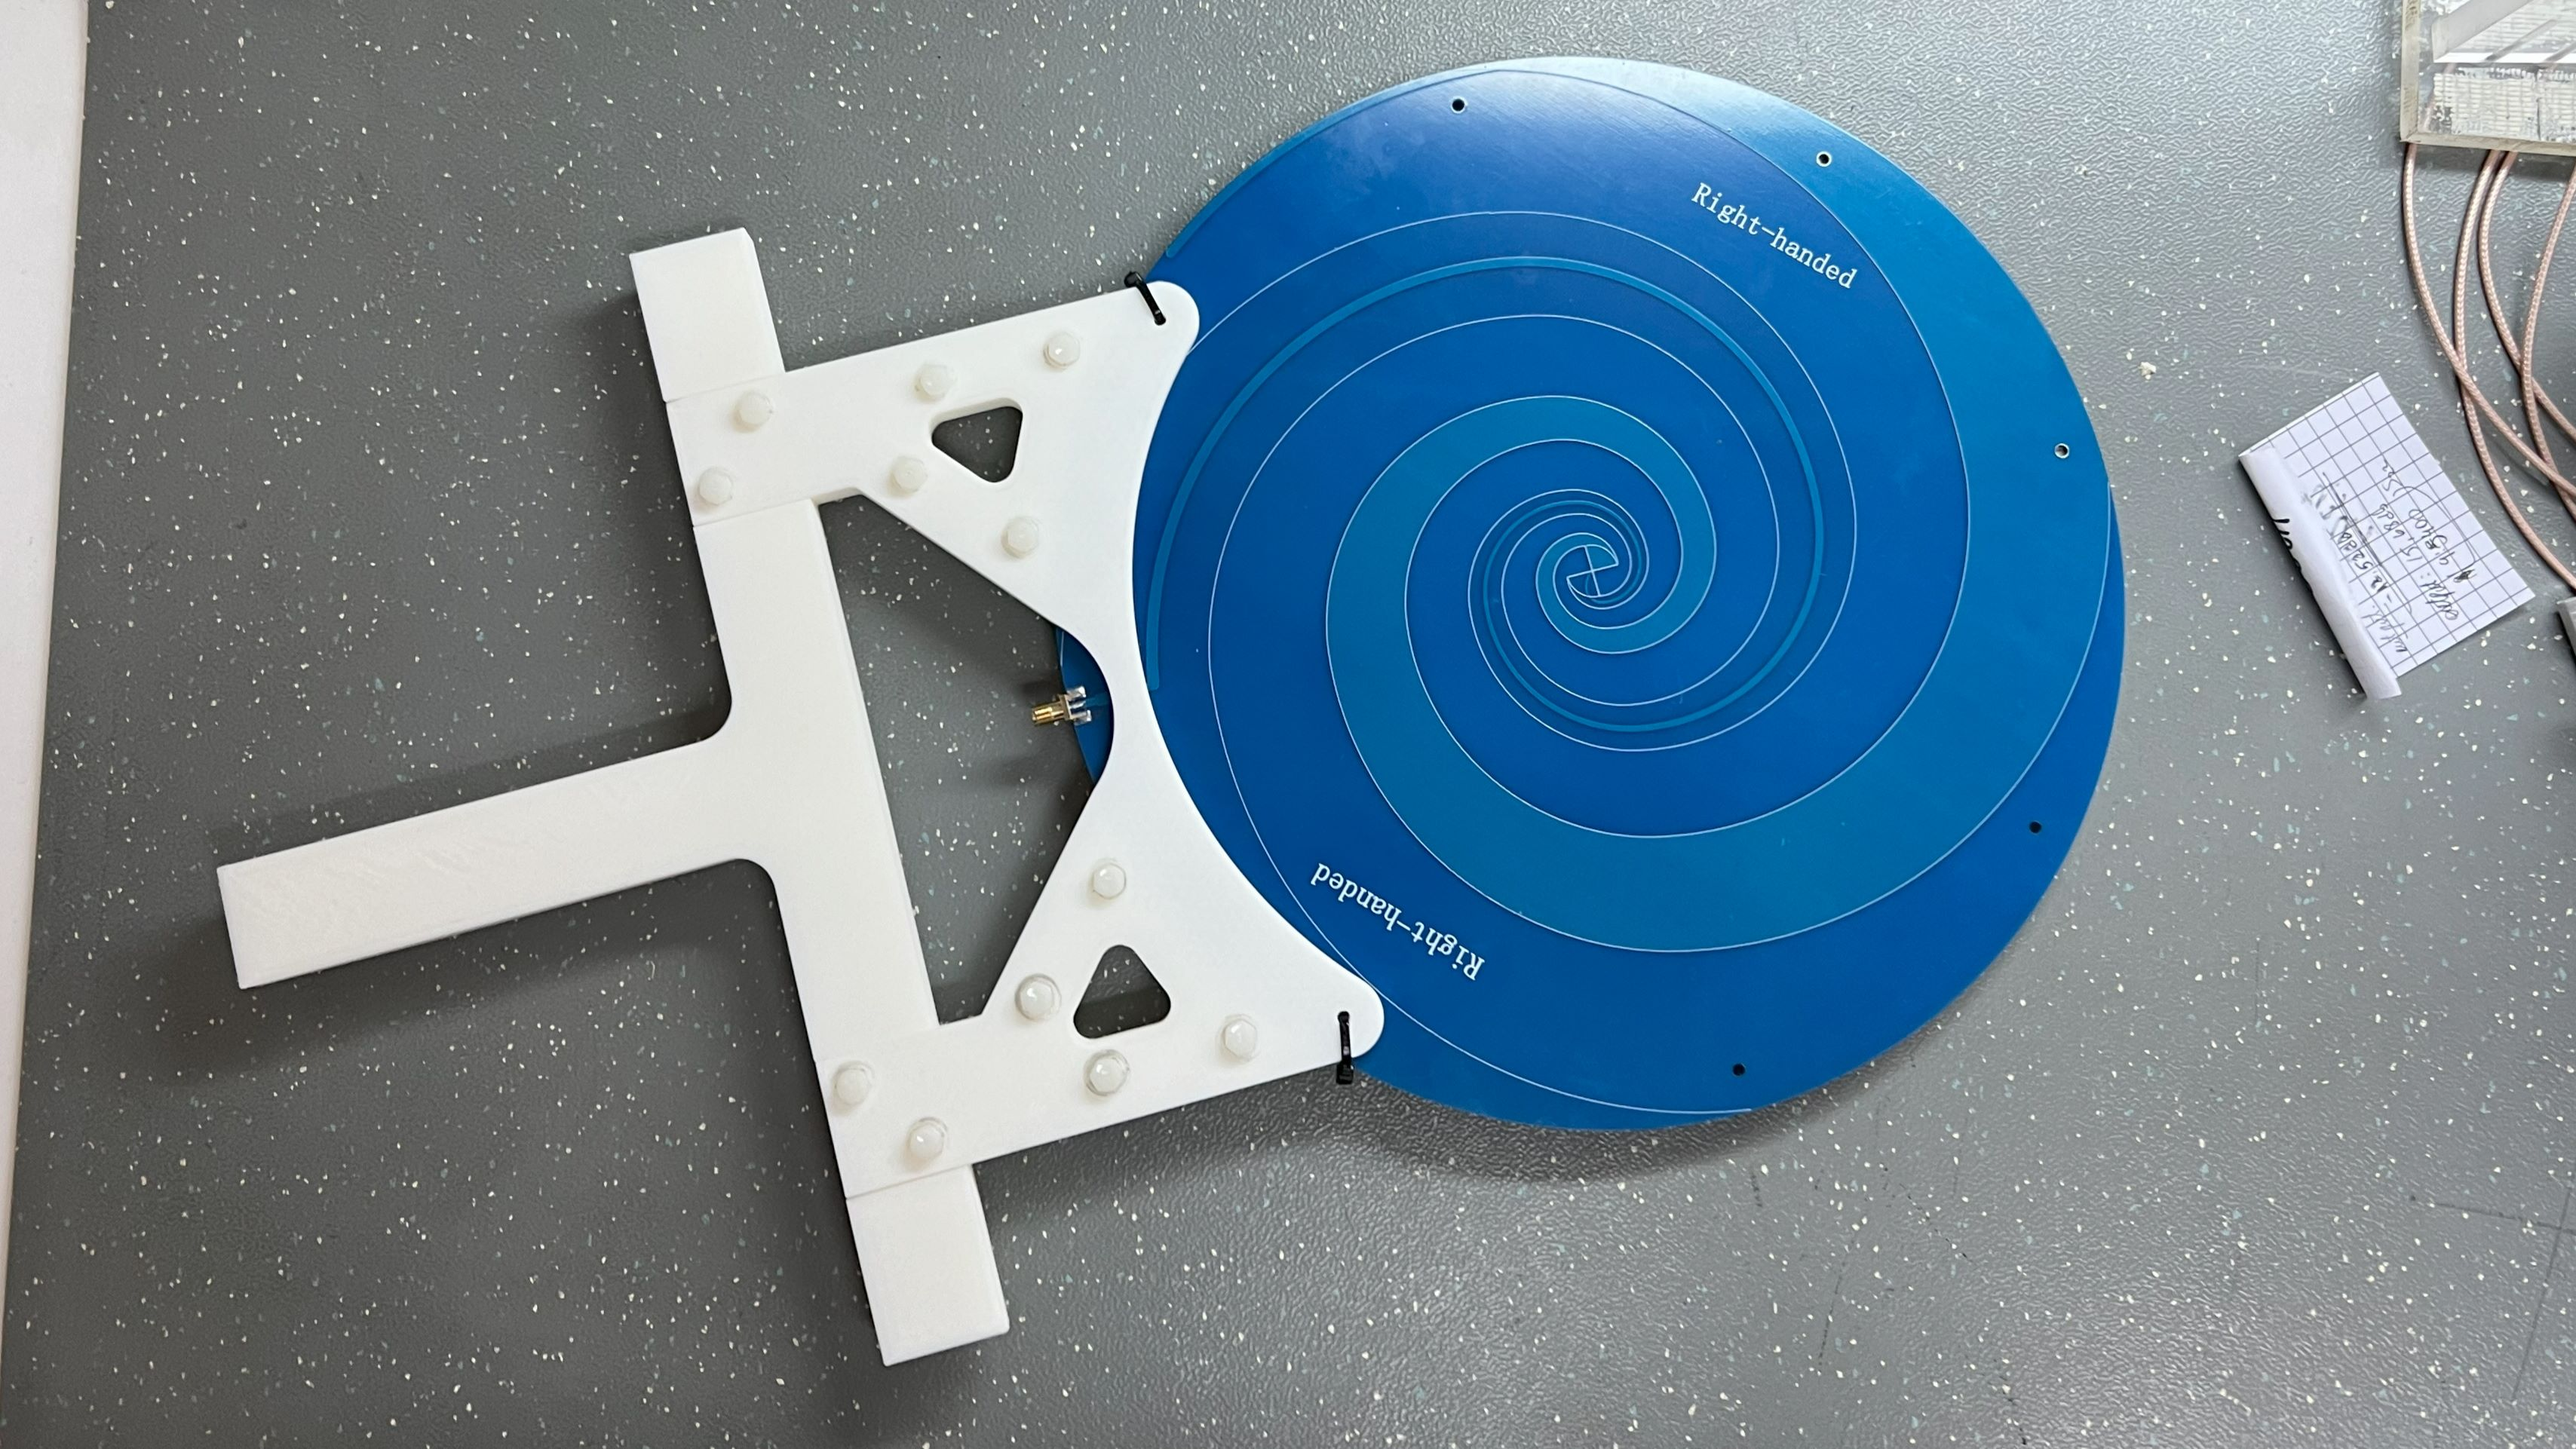
\includegraphics[width=\textwidth]{img/paleta}
        \caption{Antena de polarizacion circular de alto ancho de banda con su soporte para la copa de agua.}
        \label{fig:antena_estrella}
    \end{subfigure}
    \begin{subfigure}{0.45\textwidth}
        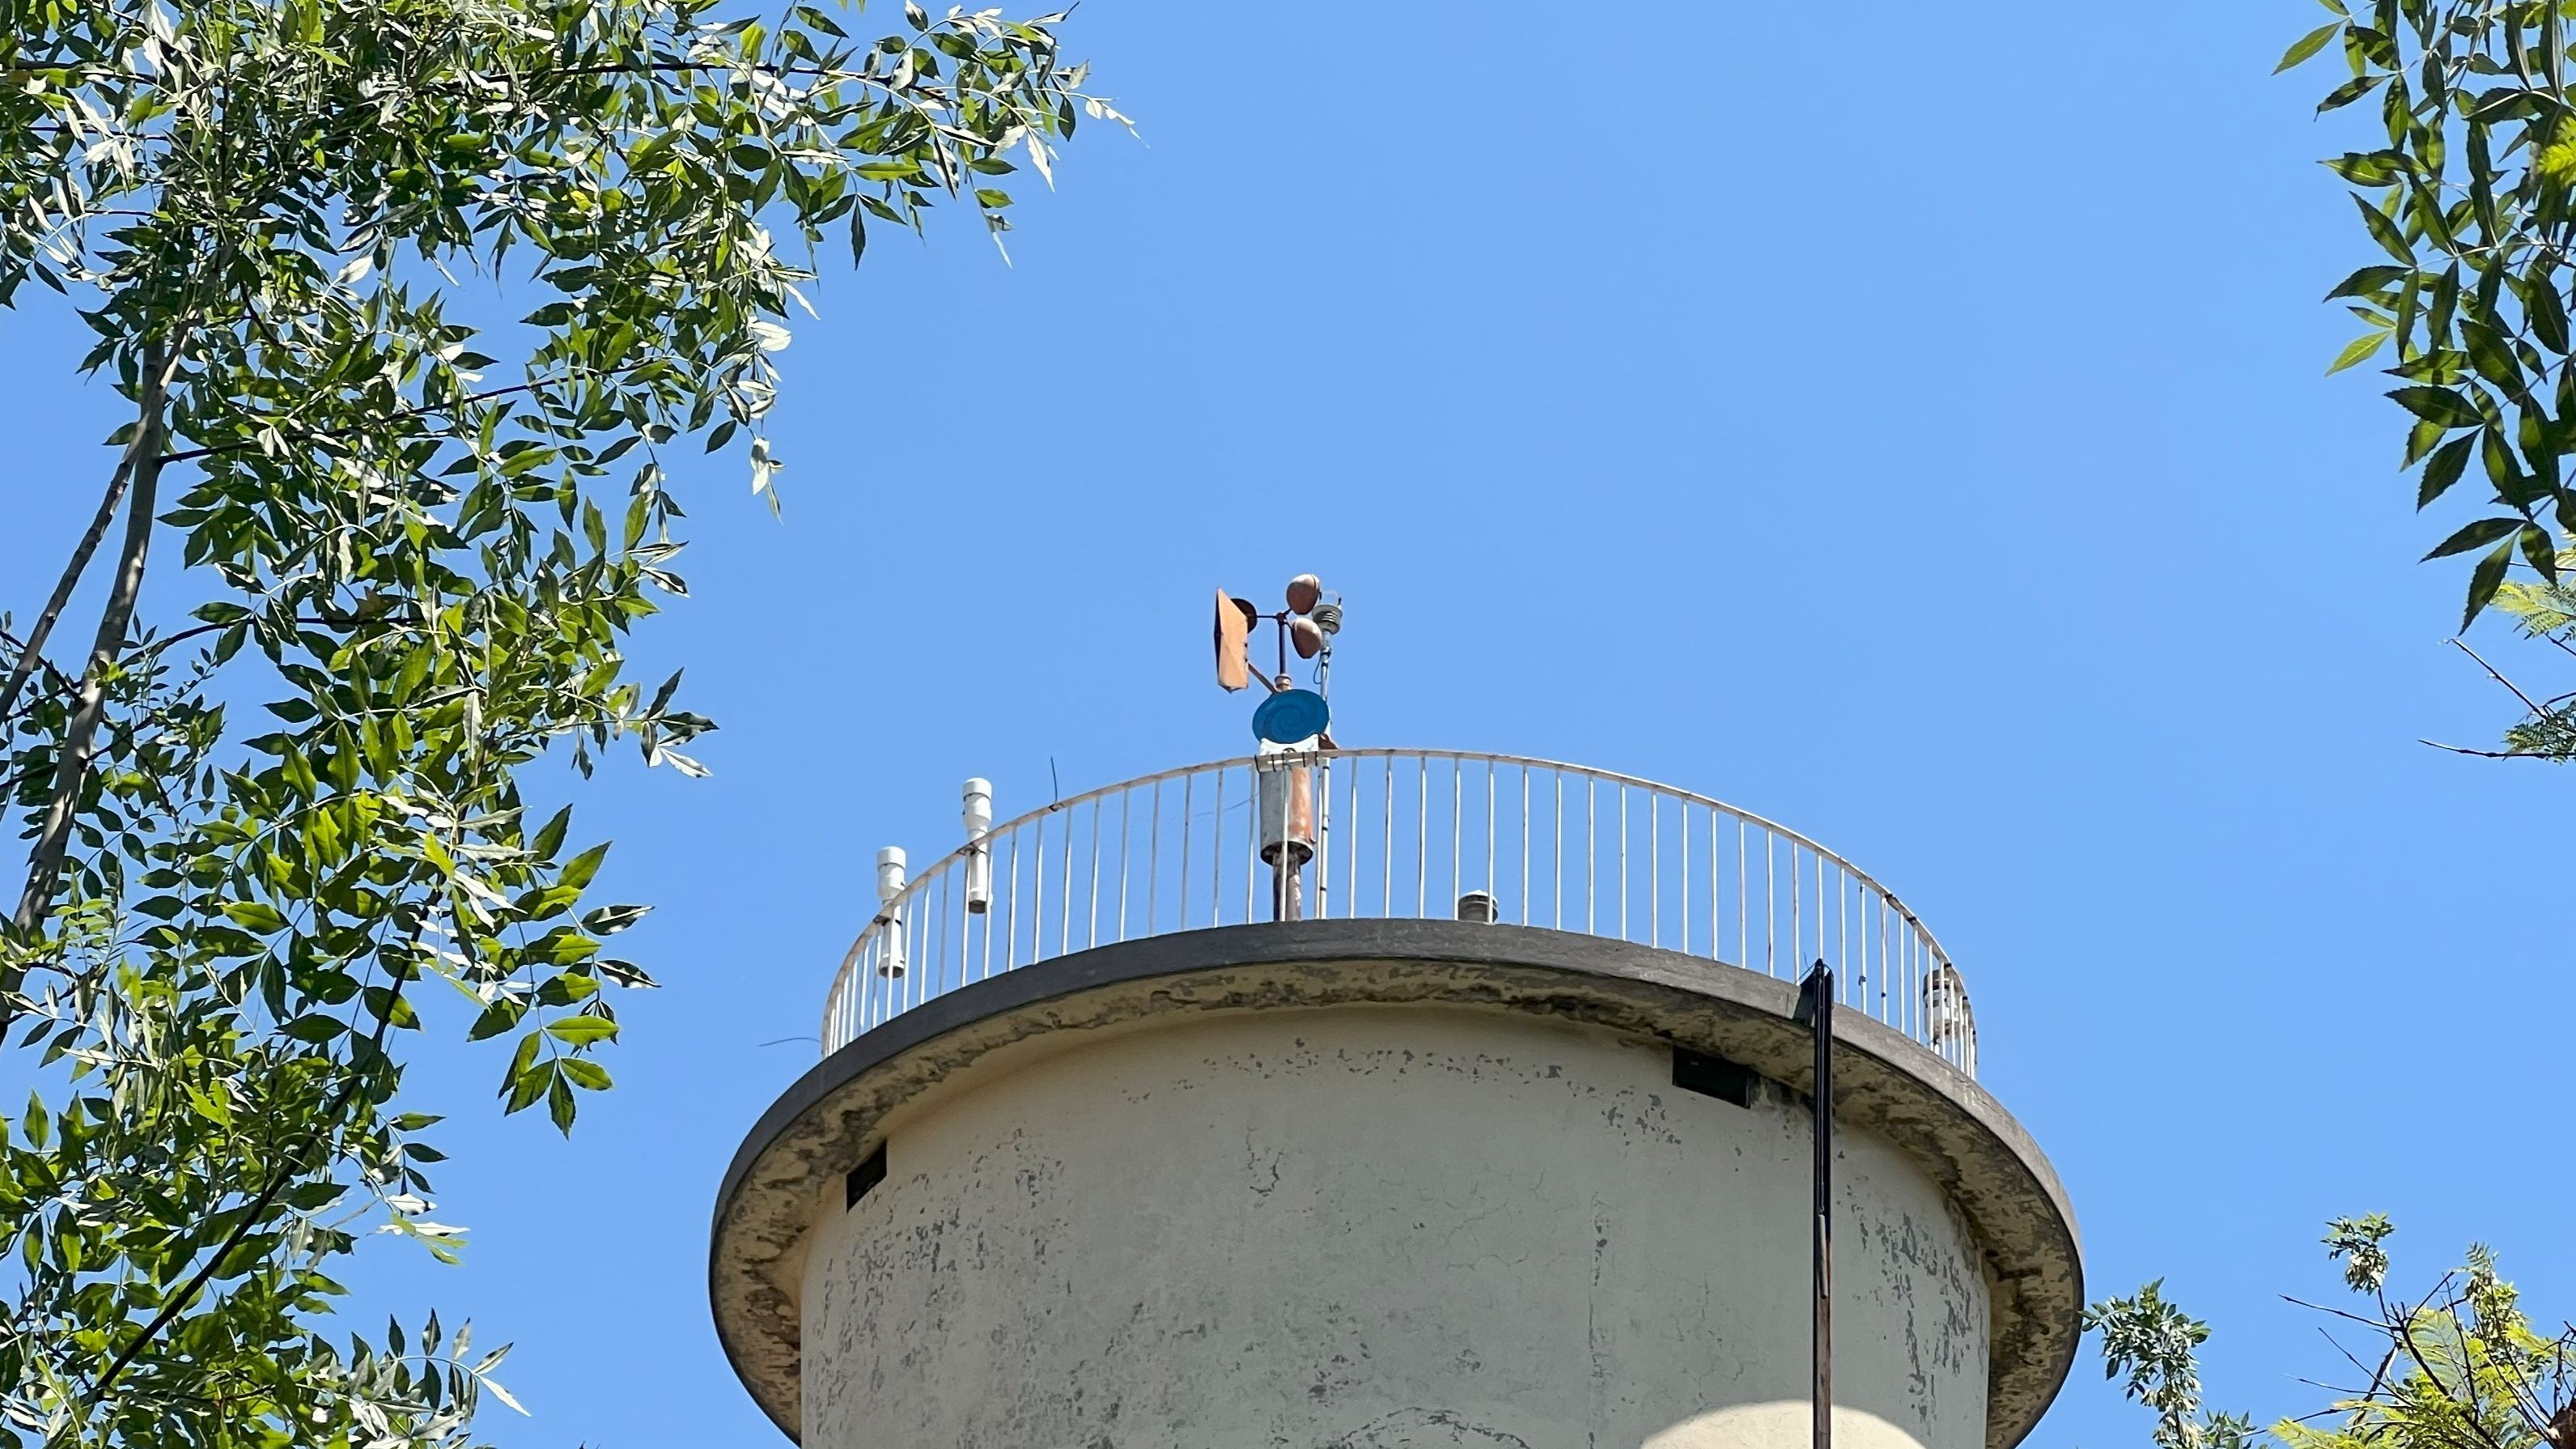
\includegraphics[width=\textwidth]{img/fake_star}
        \caption{Antena de la estrella artificial instalada en la copa de agua.}
        \label{fig:antena_estrella2}
    \end{subfigure}
\end{figure}

La antena de la estrella artificial se encuentra a una altura de 15 metros sobre el suelo y a 186 metros de la antena del telescopio. La antena de la estrella artificial es una antena de polarizacion circular de alto ancho de banda con una ganancia de 3 dBi aproximadamente.\\

La línea de vista de la antena se encuentra totalmente despejada, manteniendo la primera zona de Fresnel libre de obstaculos para las frecuencias de interes.\\

Como generador se señales se utilizo un generador Valon 5008 con una salida de 2.23 dBm a 1428 MHz y a 400MHz. Ademas se le isntalo un filtro pasabajo para minimizar la presencia de los armonicos de alta frecuencia evitando la generacion innecesaria de RFI.\\

\begin{figure}
    \centering
    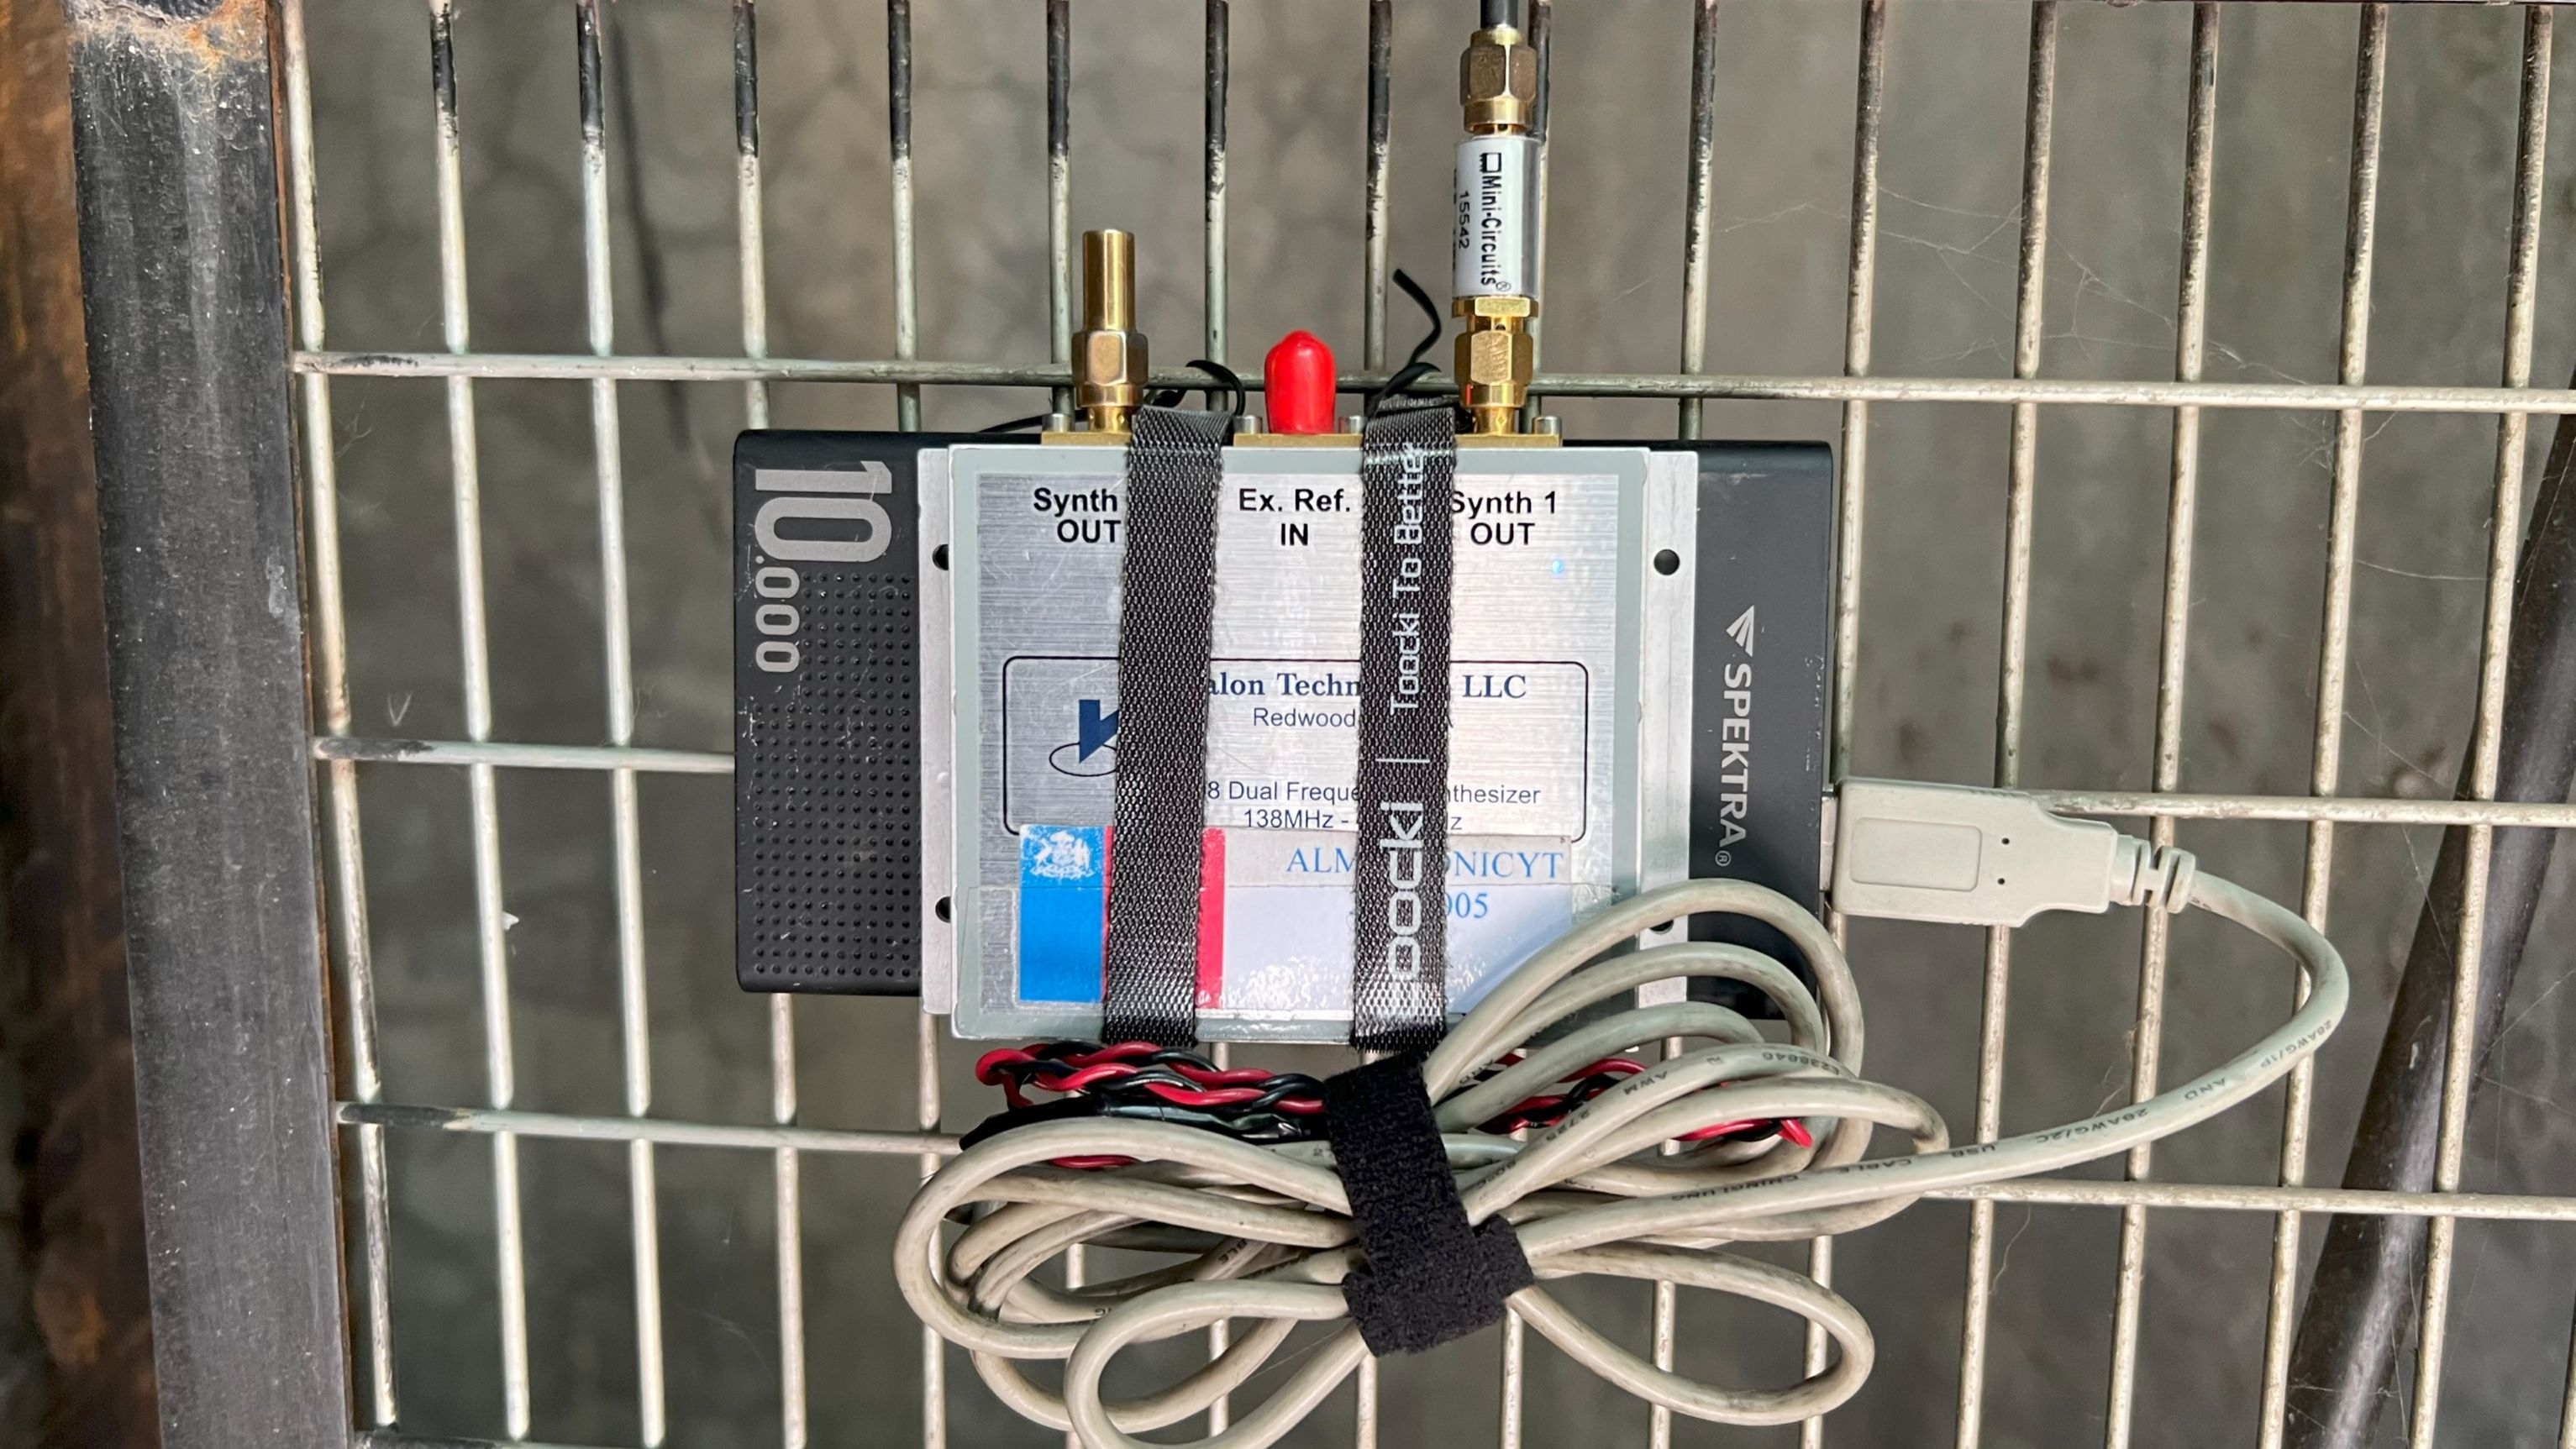
\includegraphics[width=0.8\textwidth]{img/valon}
    \caption{Generador de señales Valon 5008 con filtro pasabajo con una bateria externa.}
    \label{fig:generador}
\end{figure}

El generador de la figura \ref{fig:generador} se conecta a la antena de la estrella artificial por medio de un cable coaxial de 20 metros de longitud y se alimenta por una bateria externa de 5 V1. Se programa previamente la frecuencia a la que se requiera para las mediciones.\\

\subsection{Fuente de ruido}

Para realizar medicion de la temperatura de ruido se requiere de una fuente de ruido. Para obtener la temperatura de la cadena de recepcion se utilizo una fuente de ruido Agilent 346B con una aliemntacion de 28 V.\\

\begin{figure}
    \centering
    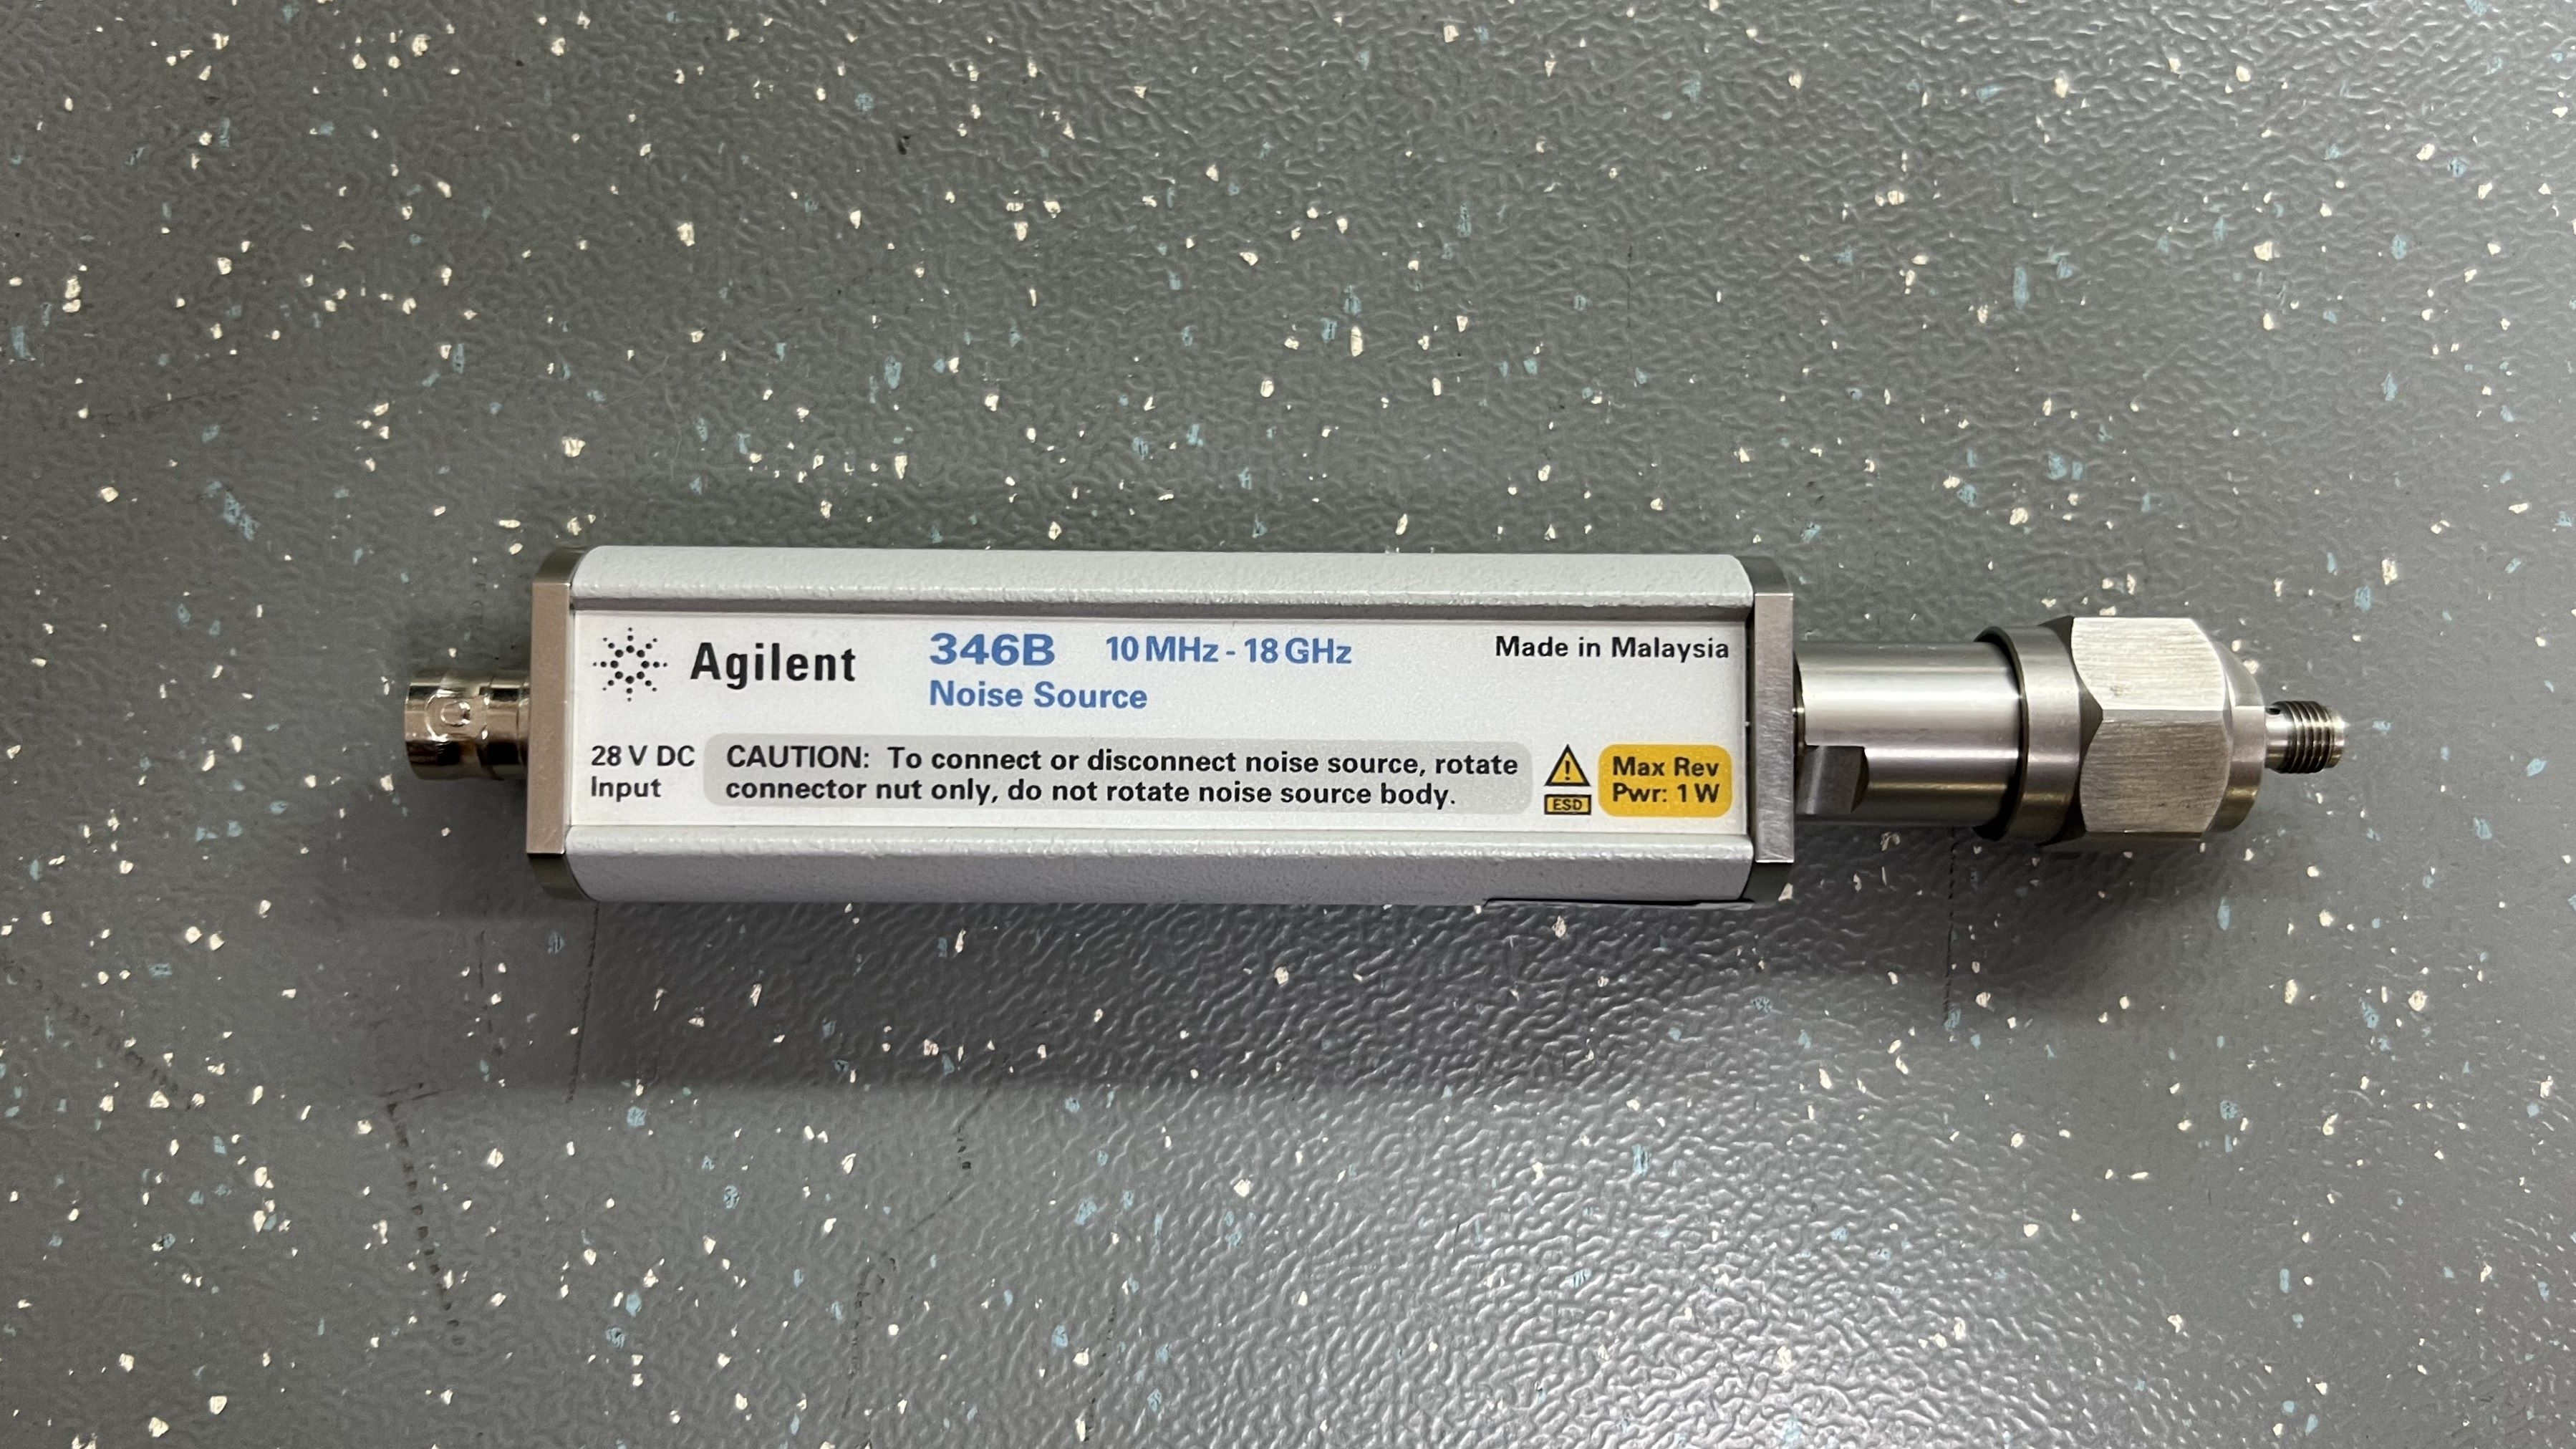
\includegraphics[width=0.8\textwidth]{img/fuenteRuido}
    \caption{Fuente de ruido Agilent 346B.}
    \label{fig:fuente_ruido}
\end{figure}

\subsection{Software de caracterización}

\paragraph{cpt\_rp\_measure.py} Es un software que al igual que los de la seccion \ref{sec:software} obtiene espectros y los guarda para el analisis futuro. La diferencia es que este software esta diseñado para la calibracion del instrumento, por lo que ademas este instrumento guardas los espectros tomados por angulo con respecto a la estrella artificial de la copa de agua para las mediciones de patron de radiacion.\\

Este script genera un archivo con los espectros tomados por angulo y luego mueve la montura a otro angulo para tomar otro espectro, este proceso se repite hasta que se obtienen un corte de 180 grados con la cantidad de espectros que haya sido configurada.\\

Como la fuente de calibracion se encuentra en altura, hay que ajustar el plano de rotacion con respecto a plano azmutal de la montura, para esto se utiliza la siguiente conversion de coordenadas:\\

\begin{equation}
    \theta' = \theta + \left(1- \frac{2\phi}{\pi}\right)E
\end{equation}

\begin{equation}
    \phi' = \phi
\end{equation}

Donde $\theta$ es la elevacion original, $E$ es el angulo de elevacion de la estrella artificial con respecto a la antena, $\phi$ es el azimut, $\theta'$ y $\phi'$ son las nuevas coordenadas. Con esta conversion se tiene una elevacion específica para cada punto de azimut que permite mantener el plano de rotacion de la fuente de calibracion en el nuevo plano de azimutal.\\

\paragraph{cpt\_siglent.py} ES un software que utiliza de manera remota el instrumento Siglent SVA1075X para obtener sus espectros y realizar las mismas mediciones de patron de radiacion que el software anterior.\\